\documentclass[pdflatex,11pt]{aghdpl}
% \documentclass{aghdpl}               % przy kompilacji programem latex
% \documentclass[pdflatex,en]{aghdpl}  % praca w języku angielskim
\usepackage[polish]{babel}
\usepackage[utf8]{inputenc}
\usepackage{listings}
\usepackage[T1]{fontenc}

% dodatkowe pakiety
\usepackage{enumerate}
\usepackage{listings,color}
\lstloadlanguages{TeX}

\lstset{
  literate={ą}{{\k{a}}}1
           {ć}{{\'c}}1
           {ę}{{\k{e}}}1
           {ó}{{\'o}}1
           {ń}{{\'n}}1
           {ł}{{\l{}}}1
           {ś}{{\'s}}1
           {ź}{{\'z}}1
           {ż}{{\.z}}1
           {Ą}{{\k{A}}}1
           {Ć}{{\'C}}1
           {Ę}{{\k{E}}}1
           {Ó}{{\'O}}1
           {Ń}{{\'N}}1
           {Ł}{{\L{}}}1
           {Ś}{{\'S}}1
           {Ź}{{\'Z}}1
           {Ż}{{\.Z}}1
}

\definecolor{gray}{rgb}{0.4,0.4,0.4}
\definecolor{darkblue}{rgb}{0.0,0.0,0.6}
\definecolor{cyan}{rgb}{0.0,0.6,0.6}

\lstset{
  basicstyle=\ttfamily,
  columns=fullflexible,
  showstringspaces=false,
  commentstyle=\color{gray}\upshape
}
 
\lstdefinelanguage{XML}
{
  basicstyle=\ttfamily\color{darkblue}\bfseries,
  morestring=[b]",
  morestring=[s]{>}{<},
  morecomment=[s]{<?}{?>},
  stringstyle=\color{black},
  identifierstyle=\color{darkblue},
  keywordstyle=\color{cyan},
  morekeywords={xmlns,version,type}% list your attributes here
}
%---------------------------------------------------------------------------

\author{Krzysztof Wilaszek~Tomasz Wójcik}
\shortauthor{K. Wilaszek~T. Wójcik}
%\author{Tomasz Wójcik}
%\shortauthor{T. Wójcik}

\titlePL{Analiza narzędzi dla zarządzania mechanizmami bezpieczeństwa w aplikacjach o charakterze SOA w środowiskach wielodomenowych}
\titleEN{Tools analysis for security management of SOA applications in multi-domain environements}

\shorttitlePL{Analiza narzędzi dla zarządzania mechanizmami bezpieczeństwa w aplikacjach o charakterze SOA w środowiskach wielodomenowych} % skrócona wersja tytułu jeśli jest bardzo długi
\shorttitleEN{Tools analysis for security management of SOA applications in multi-domain environements}

\thesistypePL{Praca magisterska}
\thesistypeEN{Master of Science Thesis}

\supervisorPL{dr inż. Marcin Jarząb}
\supervisorEN{Marcin Jarząb Ph.D}

\date{2013}

\departmentPL{Katedra Informatyki}
\departmentEN{Department of Computer Science}

\facultyPL{Wydział Informatyki, Elektroniki i Telekomunikacji}
\facultyEN{Faculty of Computer Science, Electronics and Telecommunications}

\acknowledgements{Serdecznie dziękuję \dots prowadzącemu pracownię projektową!}



\setlength{\cftsecnumwidth}{10mm}

%---------------------------------------------------------------------------

\begin{document}

\titlepages

\tableofcontents
\clearpage

\chapter{Wprowadzenie}
\label{cha:wprowadzenie}

\LaTeX~jest systemem składu umożliwiającym tworzenie dowolnego typu dokumentów (w~szczególności naukowych i technicznych) o wysokiej jakości typograficznej (\cite{Dil00}, \cite{Lam92}). Wysoka jakość składu jest niezależna od rozmiaru dokumentu -- zaczynając od krótkich listów do bardzo grubych książek. \LaTeX~automatyzuje wiele prac związanych ze składaniem dokumentów np.: referencje, cytowania, generowanie spisów (treśli, rysunków, symboli itp.) itd.

\LaTeX~jest zestawem instrukcji umożliwiających autorom skład i wydruk ich prac na najwyższym poziomie typograficznym. Do formatowania dokumentu \LaTeX~stosuje \TeX a (wymiawamy 'tech' -- greckie litery $\tau$, $\epsilon$, $\chi$). Korzystając z~systemu składu \LaTeX~mamy za zadanie przygotować jedynie tekst źródłowy, cały ciężar składania, formatowania dokumentu przejmuje na siebie system.

%---------------------------------------------------------------------------

\section{Cele pracy}
\label{sec:celePracy}

Celem poniższej pracy jest zapoznanie studentów z systemem \LaTeX~w zakresie umożliwiającym im samodzielne, profesjonalne złożenie pracy dyplomowej w systemie \LaTeX.


%---------------------------------------------------------------------------

\section{Zawartość pracy}
\label{sec:zawartoscPracy}

W rodziale~\ref{cha:pierwszyDokument} przedstawiono podstawowe informacje dotyczące struktury dokumentów w \LaTeX u. Alvis~\cite{Alvis2011} jest językiem 



















\chapter{Analiza dziedziny problemu}
\label{cha:analizaDziedzinyProblemu}

%---------------------------------------------------------------------------

\section{Koncepcja cyfrowego zarządzania tożsamościami(IdM)}
\label{sec:konceptcjaIdM}

	Zarządzanie tożsamościami(Identity Management) jest podejściem do zagadnienia zapewnienia bezpieczeństwa dostępu do aplikacji w oparciu o dane identyfikujące użytkownika(Identity). Pojęcie danych identyfikujących może być zdefiniowane jako ,,informacje o jednostce pozwalające na identyfikację tej jednostki dla pewnej dziedziny zastosowań''\cite{Itu09}. W kontekście systemów zarządzania cyfrowymi tożsamościami dane identyfikujące mogą dotyczyć nie tylko osób ale również na przykład komponentów programowych\cite{Bertino11}. Zgodnie z rekomendacją Y.2720 w skład danych identyfikujących wchodzą identyfikator jednostki, dane uwierzytelniające jednostkę oraz atrybuty opisujące jednostkę\cite{Itu09}.

	Elisa Bertino i Kenji Takahashi w książce ,,Identity Management'' definiują cele zarządzania tożsamościami jako ,,utrzymanie integralności danych identyfikujących w trakcie ich użytkowania w celu udostępniania tych danych i powiązanych z nimi informacji w sposób bezpieczny i chroniący prywatność użytkowników''\cite{Bertino11}.
	 
	\subsection{Role w koncepcji systemów zarządzania tożsamościami}

		Systemy zarządzania tożsamościami charakteryzują się rozdzieleniem odpowiedzialności związanych z dostarczaniem funkcjonalności oraz zadań związanych z zapewnieniem bezpieczeństwa dostępu do aplikacji. Usługi uwierzytelniania i autoryzacji oraz funkcjonalności systemów dostarczane są dla jednostek - składowych systemu zarządzania tożsamościami - zazwyczaj użytkowników.
		Dane identyfikacyjne jednostek są gromadzone i wykorzystywane w trakcie korzystania z aplikacji. Dane osobowe mogą obejmować informacje związane z dokumentami tożsamości(numery dowodu osobistego, paszportu), dane bankowe, biometryczne oraz informacje związane z przebiegiem interakcji jednostki z systemem. Dane identyfikacyjne jednostek powinny być przetwarzane i gromadzone w sposób zapewniający  ochronę przed niewłaściwym użyciem. Nadużycia danych osobowych jednostek mogą prowadzić do istotnych strat użytkowników aplikacji.
		Elementem przeprowadzającym weryfikację tożsamości jednostek jest usługa ,,Identity Provider''(IdP). Usługa ta odpowiedzialna jest za przyporządkowywanie jednostkom atrybutów opisujących tożsamość, tworzenie powiązań pomiędzy różnymi atrybutami jednostki oraz tworzenie asercji zawierających informacje o atrybutach jednostek. 

		Usługa 'Identity Provider' może współpracować z innymi usługami tego typu dołączając do danych uwierzytelniających informacje udostępniane przez inne zaufane usługi IdP. Wykorzystanie danych uwierzytelniających dostarczanych przez inne usługi uwierzytelniające wymaga wprowadzenia procesu zapewnienia wiarygodności otrzymywanych danych. Proces ten może opierać się na przypisywaniu miary wiarygodności do atrybutów uwierzytelniających. Wyznaczenie wartości tej miary może być na przykład oparte o ocenę stopnia zaawansowania mechanizmów weryfikacji danych uwierzytelniających wykorzystywanych przez usługę dostarczająca dany atrybut tożsamości.

		Dostawcy usług wykorzystujący infrastrukturę systemów zarządzania tożsamościami przed zezwoleniem na dostęp do swoich zasobów zlecają usługom typu IdP przeprowadzenie procesu uwierzytelniania klienta na podstawie otrzymanych danych uwierzytelniających. Dostawcy usług powinni mieć możliwość deklaracji poziomu skuteczności zabezpieczeń wykorzystywanych w procesie autoryzacji dostępu do określonych zasobów. Poziom ten może być różny w zależności od rodzaju zasobu.

		Przedstawiona w książce ,,Identity Management Concepts, Technologies, and Systems'' terminologia wprowadza również pojęcie jednostki nadzorującej\cite{Bertino11}. Jest to najczęściej instytucja upoważniona prawnie do nadzoru nad procesami przetwarzania i przechowania danych osobowych lub wglądu  w informacje o charakterze poufnym.

	\subsection{Relacje miedzy rolami w systemach zarządzania tożsamościami}

		\begin{figure}[h]
			\centering
			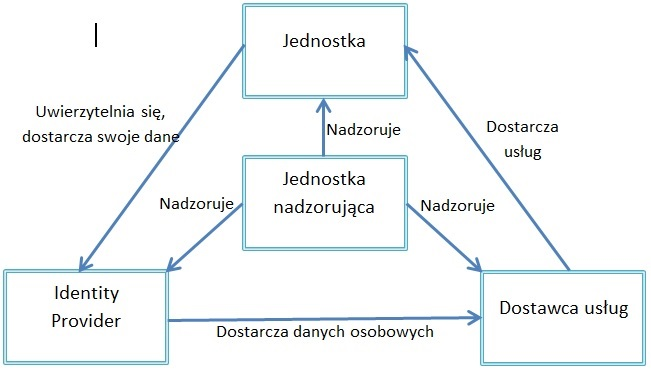
\includegraphics[width=15cm]{img/idmRelations.jpg}
			\caption{Relacje miedzy rolami w systemach zarządzania tożsamościami}
			\label{Relacje miedzy rolami w systemach zarządzania tożsamościami}
		\end{figure}

		Często stosowanym modelem jest infrastruktura złożona z jednej usługi typu ,,Identity Provider'' oraz wielu usług funkcjonalnych opierających na niej swoje mechanizmy zabezpieczeń. Dzięki takiemu rozwiązaniu dostawcy usług mogą skoncentrować się na tworzeniu funkcjonalności stanowiących istotę aplikacji - odpowiedzialności związane z zapewnieniem bezpieczeństwa dostępu delegowane są do usługi IdP. Specjalizowana usługa uwierzytelniania może dostarczać bardziej zaawansowanych zabezpieczeń. Dzięki realizacji tego modelu użytkownicy nie muszą zarządzać wieloma danymi uwierzytelniającymi dla różnych usług - dostęp do wielu serwisów gwarantowany jest przy użyciu tych samych danych. Wprowadza to jednak zagrożenia związane z centralizacja dostępu do różnych usług.

	\subsection{Federated Identity Management}

		Najczęściej użytkownicy korzystają nie z jednej usługi lecz z szerokiej gamy różnych usług. Każda z usług korzysta z własnych danych uwierzytelniających. Podejście ,,Federated Identity Management'' umożliwia tworzenie powiązań pomiędzy tożsamościami użytkownika w ramach różnych usług dzięki czemu dane uwierzytelniające każdej z sfederowanych usług mogą być wykorzystane w procesie uwierzytelniania dowolnej z usług.

	\subsection{Cykl życia tożsamości}

		Jednym z głównych zadań systemów zarządzania tożsamościami jest kontrola nad cyklem życia tożsamości. Autorzy książki ,,Identity Management: Concepts, Technologies and Systems'' opisują 4 etapy cyklu życiu tożsamości: tworzenie, użytkowanie, aktualizacja oraz wycofanie z użycia\cite{Bertino11}.

		Proces tworzenia cyfrowej tożsamości składa się z kilku kroków. Pierwszym z nich może być weryfikacja przedstawionych atrybutów tożsamości, wymagająca udowodnia przez jednostkę prawdziwości wprowadzanych danych. Następnie tworzone są dane uwierzytelniające. Ostatnim krokiem jest utworzenie tożsamości na podstawie otrzymanych danych oraz nadanie jednostce identyfikatora.

		Utworzona tożsamość może być wykorzystywana w różnych celach, np. zapewnienia wiarygodnej komunikacji lub w procesie jednokrotnego uwierzytelniania(ang. Single Sign-On).

		Systemy zarządzania tożsamościami powinny obsługiwać zmiany atrybutów tożsamości. Powinny aktualizować informacje o danych jednostek po zmianach wysyłając powiadomienia do usług przechowujących te dane, np. ,,Identity Provider''. Identyfikatory jednostek nie powinny podlegać zmianom. Systemy IdM muszą również usuwać tożsamości jeśli nie są już aktualne.

\section{Jednokrotne uwierzytelnianie}

	Książka ,,Identity Management: Concepts, Technologies and Systems'' definiuje jednokrotne uwierzytelnianie(ang. Single Sign-On) jako proces uwierzytelniania, w którym jednostka może wykorzystać wynik pojedynczego uwierzytelniania dla uzyskania dostępu do wielu niezależnych usług z ochroną dostępu\cite{Bertino11}. 

	Podstawą funkcjonowania mechanizmów jednokrotnego uwierzytelniania jest nawiązanie relacji zaufania pomiędzy dostawcami usług oraz serwisami typu ,,Identity Provider''. Po uwierzytelnieniu użytkownika w ramach jednej z usług objętych mechanizmem SSO dostęp do innej nie wymaga uwierzytelniania - dane uwierzytelniające są mapowane na dane niezbędne do uwierzytelnienia względem innej usługi oraz generowane są informacje pozwalające na uzyskanie dostępu do serwisu. Usługi korzystające z mechanizmu jednokrotnego uwierzytelniania powinny otrzymywać informacje kontekstowe o przebiegu procesu uwierzytelniania takie jak: wykorzystywane metody uwierzytelniania oraz sposób ochrony danych uwierzytelniających. Informacje te pozwalają na ocenę stopnia wiarygodności przeprowadzonego procesu uwierzytelniania.

	\subsubsection{Architektura systemów jednokrotnego uwierzytelniania}

		Implementacja mechanizmu jednokrotnego uwierzytelniania może opierać się o różne architektury. Autorzy książki ,,Identity Management: Concepts, Technologies and Systems''\cite{Bertino11} wymieniają następujące typy architektur systemów jednokrotnego uwierzytelniania:

		\begin{itemize}
		  \item Architektura oparta o brokery - architektura składająca się z punktu centralnego(serwera) oraz jednostek przez niego uwierzytelnianych. Serwer przydziela użytkownikom tokeny uwierzytelniające, dzięki którym możliwy jest dostęp do aplikacji. Przykładem architektury tego typu jest protokół Kerberos. 
		  \item Architektura oparta o agenty - architektura, w której w dostępie do każdej aplikacji pośredniczy agent uwierzytelniania. Jego rolą jest translacja pomiędzy metodą uwierzytelniania zastosowaną przez klienta a mechanizmami obsługiwanymi przez aplikację.
		  \item ,,Reverse proxy-based architecture'' - architektura wprowadzająca usługę proxy pośredniczącą w dostępie do wszystkich aplikacji objętych procedurą SSO. Moduł proxy dokonuje filtrowania przychodzących komunikatów - nieuwierzytelnione żądania zostają przekierowane, np. do serwera uwierzytelniającego.
		\end{itemize}
		  
		Procedura jednokrotnego uwierzytelniania pozwala na wygodniejszy sposób korzystania z aplikacji - znosi konieczność wielokrotnego wprowadzania danych identyfikujących. Użytkownik nie musi też zapamiętywać wielu haseł dla różnych usług. Wiele prostych haseł może zostać zastąpionych jedną bardziej wiarygodną metodą uwierzytelniania(np. z wykorzystaniem bardziej skomplikowanego hasła). Wadą wprowadzenia procedury jednokrotnego uwierzytelniania jest jednak centralizacja punktu dostępu do różnych aplikacji - złamanie zabezpieczeń otworzy drogę do wielu usług użytkownika.

%---------------------------------------------------------------------------

\section{Service-Oriented Architecture}
\label{sec:soa}

	Architektura zorientowana na usługi(ang. Service-Oriented Architecture) to architektura systemów informatycznych oparta o strukturę luźno powiązanych, rozproszonych usług, które mogą być wielokrotnie wykorzystywane i łączone w celu realizacji wymagań stawianych aplikacji. Architektura zorientowana na usługi umożliwia integrację usług w złożone procesy\cite{Lawler08}. Usługi składające się na architekturę SOA udostępniają swoje  funkcjonalności w ramach zdefiniowanych interfejsów i są od siebie niezależne. Komunikacja pomiędzy serwisami odbywa się poprzez wywołania dostarczanych przez nie operacji\cite{Papazoglou07}. 

	Architektura SOA zaprojektowana została jako rozwiązanie wielu problemów pojawiających się w trakcie tworzenia systemów rozproszonych. Do problemów tych należą: integracja aplikacji, zarządzanie transakcjami, zapewnienia bezpieczeństwa wykonywanych operacji, różnorodność środowisk uruchamiania aplikacji\cite{Papazoglou07}.

	Jednym z głównych założeń architektury zorientowanej na usługi jest niezależność od technologii implementacji. Jest to możliwe dzięki wykorzystaniu standardowych interfejsów usług oraz metod komunikacji pomiędzy nimi. Usługi w architekturze SOA są autonomiczne, same przechowują swój stan. W architekturze SOA wszelkie funkcjonalności są udostępniane w postaci usług.
	
	\subsection{Model architektury zorientowanej na usługi}
	
		Model SOA definiuje charakterystyczne elementy architektury - komponenty, usługi i przetwarzanie informacji pomiędzy nimi - realizujące określone procesy biznesowe. Model ma budowę warstwową. Definicja warstw modelu ma na celu bardziej precyzyjne odwzorowanie pomiędzy wymaganiami biznesowymi, modelowaniem funkcjonalności a realizacją konkretnych rozwiązań dla stawianych wymagań. Kluczową cecha charakterystyczną dla architektury SOA jest wyraźny rozdział pomiędzy interfejsem opisującym usługę a jej implementacją. Model architektury SOA umożliwia wydzielenie części odpowiedzialnych za poszczególne typy zadań oraz upraszcza proces projektowania i tworzenia aplikacji opartych o architekturę zorientowaną na usługi. 

		Model architektury SOA składa się z dwóch typów warstw. Warstwy oznaczone na rysunku przy pomocy bloków poziomowych ilustrują cechy funkcjonalne rozwiązań architektury SOA. Bloki pionowe przedstawiają cechy niefunkcjonalne odnoszące się do warstw funkcjonalnych. Model wprowadza rozgraniczenie pomiędzy dostawcami oraz konsumentami usług. Model zakłada powiązanie relacjami biznesowymi pomiędzy obydwoma grupami. Wyraźne rozdzielenie pomiędzy dostawcami i konsumentami usług pozwala określić kompetencje i wymagania stawiane obydwu rolom w architekturze SOA. 

	\subsection{Enterprise Service Bus} 

		W istniejących środowiskach dostarczania usług występuje często duża niejednorodność technologii, protokołów komunikacji i modeli wykorzystywanych przez różne serwisy. Jednym z rozwiązań tego problemu jest wprowadzenie warstwy pośredniczącej, która implementuje logikę pozwalającą na integrację różnorodnych usług. Rozwiązanie to stanowi podstawę dla koncepcji magistrali usług(ang. Enterprise Service Bus). 

		\begin{figure}[h]
			\centering
			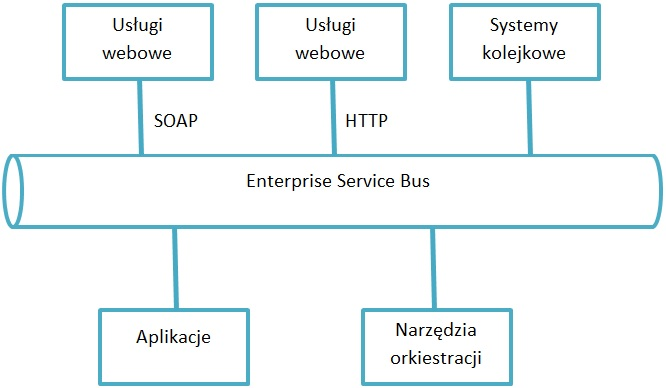
\includegraphics[width=15cm,height=8cm]{img/esb.jpg}
			\caption{Schemat funkcjonowania magistrali usług}
			\label{Schemat funkcjonowania magistrali uslug}
		\end{figure}

		Magistrala ESB dostarcza funkcjonalności rozproszonego przetwarzania oraz integracji usług opartych o standardowe mechanizmy. Funkcje transportu i transformacji wiadomości pozwalają na komunikację pomiędzy niejednorodnymi i rozproszonymi usługami. Magistrala usług może zapewniać mechanizmy bezpieczeństwa dostępu do aplikacji, wiarygodności dostarczania danych oraz audytu komunikacji. ESB powinno pozwalać na przekazywanie informacji kontekstowych np. dotyczących transakcji lub bezpieczeństwa dostępu do usług.

		Mechanizmy ESB uniezależniają klientów usług od fizycznych właściwości dostarczania usługi. Dzięki zastosowaniu magistrali usług możliwe jest dokonywanie zmian po stronie usługi lub zastąpienie usługi inną bez wpływu na aplikację kliencką. 

	\subsection{Zarządzanie procesami biznesowymi} 

		Istnieje szereg aplikacji, które realizując swoje funkcjonalności korzystają z różnorodnych usług. W ten sposób mogą powstawać skomplikowane procesy obejmujące komunikację z wieloma komponentami programowymi jak i interakcje z użytkownikami. Dla tego typu zastosowań użyteczne jest wprowadzenie mechanizmów zarządzania procesami biznesowymi(ang. Business Process Management) - technologii zapewniającej kontrolę nad przebiegiem wieloetapowych procesów obejmujących różne usługi w środowisku wielo-domenowym.

		Narzędzie zarządzania procesami biznesowymi pozwalają na automatyzację procesów. Definicja procesów opiera się o schemat organizacji zadań(ang. workflow). Narzędzie BPM umożliwiają wizualizację, modelowanie i analizę procesów biznesowych. Zarządzanie procesami biznesowymi jest dzięki temu metodologią pozwalającą na tworzenie, przedstawianie i nadzorowanie procesów biznesowych oraz upraszcza zrozumienie przebiegu procesu. Mechanizmy BPM pozwalają na monitorowania wykonania procesu biznesowego oraz dostęp do informacji o jego statusie. 

	\subsection{Zapewnienie bezpieczeństwa dostępu do usług w architekturze SOA}

		Ważnym aspektem dostarczania usług sieciowych jest zapewnienie mechanizmów bezpieczeństwa w procesie komunikacji. Mechanizmy bezpieczeństwa mogą być włączone w warstwie transportowej procesu dostarczania usług lub mogą być realizowane na poziomie wiadomości przesyłanej pomiędzy komunikującymi się jednostkami\cite{Szychowiak09}. 

		Zabezpieczenia warstwy transportowej polegają na zestawieniu szyfrowanej komunikacji pomiędzy klientem i dostawcą usług. Dzięki temu możliwe jest zapewnienie poufności wymiany wiadomości pomiędzy uczestnikami procesu komunikacji i integralności dostarczanych danych. Możliwa jest również implementacja mechanizmów uwierzytelniania w oparciu o szyfrowanie komunikatów\cite{Kolaczek09}.

		Istnieją sytuacje, w których zabezpieczenia warstwy transportowej nie są wystarczające.  Nie pozwalają one na zapewnienie bezpieczeństwa w razie konieczności przetwarzania informacji przez węzły pośrednie. Nie umożliwiają również zapewnienia poufności jedynie fragmentu wiadomości a nie całej jej treści. Rozwiązaniem tego problemów jest zastosowanie koncepcji mechanizmów bezpieczeństwa na poziomie przesyłanych wiadomości. Koncepcja ta zakłada oparcie mechanizmów bezpieczeństwa o informacje dołączane do wiadomości wymienianych pomiędzy klientem i dostawcą usługi. Przesyłane informacje mogą pozwalać na przeprowadzenie procesu uwierzytelniania lub zapewnienie integralności komunikatów. Istnieją liczne standardy opisujące format danych dołączanych do wiadomości oraz sposób ich przesyłania przy pomocy protokołów wykorzystywanych do dostarczania usług. Standardy tego typu definiują również sposób szyfrowania wymienianych wiadomości.		
%---------------------------------------------------------------------------

\section{Wymagania stawiane systemom Business-to-Business}
\label{sec:wymaganiaB2B}

Wymagania stawiane systemom Business-to-Business

%---------------------------------------------------------------------------

\section{Zakres wymagań tworzonego systemu}
\label{sec:zakresWymagan}

	W ramach projektu implementacyjnego  związanego z niniejszą pracą przygotowano przykłady ilustrujące zastosowanie mechanizmów systemów zarządzania tożsamościami. Punktem wyjścia była implementacja mechanizmu jednokrotnego uwierzytelniania oraz jednokrotnego wylogowywania dla aplikacji z interfejsem udostępnianym poprzez przeglądarkę internetową. Głównym celem projektu jest analiza mechanizmów zarządzania tożsamościami dla architektury zorientowanej na usługi.

	Przygotowywane moduły powinny korzystać z narzędzi uwierzytelniania i autoryzacji dostarczanych przez serwer aplikacyjny. Mechanizm uwierzytelniania powinien być oparty o protokół LDAP. Jako specyfikację realizującą założenia systemów zarządzania tożsamościami wybrano standard SAML opisany w dalszej części pracy.

	Najważniejszą częścią pracy było zastosowanie koncepcji systemów zarządzania tożsamościami w architekturze SOA. Praca powinna przedstawiać propozycję rozwiązania problemów uwierzytelniania i autoryzacji dostępu do usług sieciowych. W ramach projektu wymagana jest implementacja modułów wykorzystujących uwierzytelnianie oparte o mechanizmy systemów zarządzania tożsamościami dla różnych standardów dostarczania usług webowych(np. SOAP i REST). Należy również dokonać analizy zastosowania zaproponowanych mechanizmów uwierzytelniania w architekturze zorientowanej na usługi. Powinien zostać opracowany mechanizm magistrali usług pozwalający na przekazywanie informacji uwierzytelniających pomiędzy modułami systemu. Wykorzystanie zaimplementowanych usług wraz z mechanizmami zabezpieczania dostępu powinno być przedstawione w postaci modelu procesu biznesowego. 

	Dla ilustracji opisywanych mechanizmów opracowano zestaw usług dostarczających prostych funkcjonalności realizujących różne etapy dokonywania zamówienia w sklepie internetowym(usługi sprawdzania stanu magazynu, zlecenia wydania towaru,   zlecenia transportu, rejestracji transakcji w systemie finansowym). Usługi korzystają z uwierzytelniania w systemie zarządzania tożsamościami. Usługi zaimplementowane zostały przy użyciu różnych technologii.Unifikację sposobu korzystania z serwisów osiągnięto dzięki modułowi magistrali usług. Używając zaimplementowanych usług opracowano model procesu biznesowego realizujący kompletną funkcjonalność dokonywania zamówienia.

\chapter{Przeglad dostepnych rozwiazan}
\label{cha:przegladRozwiazan}

%---------------------------------------------------------------------------

\section{Najpopularniejsze standardy IdM}
\label{sec:standardyIdM}

Implementacja systemów zarządzania tożsamościami jest obszarem, w którym standaryzacja procesów wykorzystywania danych osobowych przynosi istotne korzyści. Wprowadzenie standardowych rozwiązań upraszcza wdrożenie nowych aplikacji lub usług typu "Identity Provider". Ujednoliceniu sposobu korzystania z funkcjonalności systemów zarządzania tożsamościami umożliwia tworzenie aplikacji klienckich używających podobnych rozwiązań dla dostępu do różnych usług. Rozwijanych jest wiele standardów realizujących wymagania stawiane systemom zarządzania tożsamościami. Najbardziej istotne z nich to SAML(Security Assertion Markup Language) oraz OpenID. 

\subsection{Security Assertion Markup Language}

	SAML to oparty na języku XML standard zarządzania tożsamościami oraz wymiany informacji uwierzytelniających \cite{Wisniewski05}. SAML oparty jest na podejściu wykorzystującym federację tożsamości - umożliwia tworzenie powiązań pomiędzy różnymi cyfrowymi tożsamościami użytkownika. SAML pozwala tworzyć asercje opisujące atrybuty tożsamości jednostki oraz przekazywać je do usług wymagających informacji identyfikujących swoich klientów.

	\subsubsection{Cele technologii SAML}

		Cele stawiane technologii SAML to\cite{Wisniewski05}:

		\begin{itemize}
		  \item niezależność od platformy - mechanizmy bezpieczeństwa powinny być niezależne od środowiska i implementacji usługi.
		  \item luźne powiązanie pomiędzy elementami wchodzącymi w skład infrastruktury opartej o wymianę komunikatów SAML
		  \item uproszczenie procesu uwierzytelniania z perspektywy klienta, np. poprzez wprowadzenie procedury SSO
		  \item redukcja kosztów administracyjnych poprzez zastąpienie wielu oddzielnych modułów bezpieczeństwa jednym wspólnym dla  różnych aplikacji
		\end{itemize}

	\subsubsection{Struktura specyfikacji SAML}

		Specyfikacja technologii SAML definiuje czterowarstwową strukturę, w skład której wchodzą asercje, protokoły, mapowania dla protokołów komunikacyjnych oraz profile. 
		Asercje zawierają informacje wymieniane pomiędzy aplikacjami, usługami "Identity Provider" oraz użytkownikami. Protokoły, mapowania oraz profile definiują mechanizmy przetwarzania asercji.

		\paragraph{Asercje}\mbox{}\\
					
			Asercje są to wiadomości zawierające dane identyfikacyjne jednostek w systemie. Składają się z deklaracji tożsamości opisujących jednostki wygenerowanych przez usługę "Identity Provider" systemu SAML. Na podstawie otrzymanych deklaracji tożsamości jednostki dostawca usługi podejmuje decyzję o przyznaniu lub odmówieniu prawa dostępu do swoich zasobów. Również dostawcy usług mają możliwość tworzenia asercji w celu utworzenia zapytania do serwisu uwierzytelniającego o parametry transakcji określania tożsamości. 

			\subparagraph{Struktura asercji}\mbox{}\\
			
				\begin{figure}[h]
				\centering
					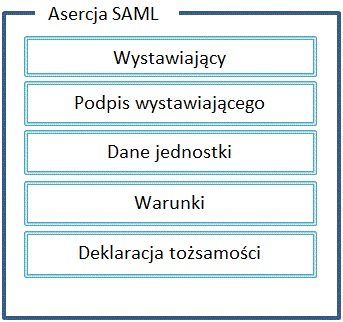
\includegraphics{img/samlAssertion.jpg}
				\caption{Elementy asercji SAML}
				\label{Elementy asercji SAML}
				\end{figure}

				Asercja SAML zawiera informacje o wystawiającym asercję. Może zawierać również informację o dacie wygenerowania asercji. W celu zapewnienia integralności informacji do asercji dołączany jest cyfrowy podpis wystawiającego. W dalszej części asercji znajdują się dane opisujące jednostkę, względem której utworzono asercję. Następną sekcją wiadomości są warunki, pod którymi asercja może być wykorzystywana. W tym fragmencie mogą znajdować się informacje o okresie ważności asercji lub usługi, do których adresowana jest asercja. Ostatnim elementem jest deklaracja tożsamości, zawierające informacje kontekstowe o procesie uwierzytelniania, np. dotyczące zastosowanej metody uwierzytelniania.

			\subparagraph{Typy deklaracji tożsamości}\mbox{}\\

				Specyfikacja definuje następujące typy deklaracji tożsamości zawartych w asercjach SAML\cite{Wisniewski05}:

				\begin{itemize}
				  \item deklaracja uwierzytelniania - stwierdza, że opisana w asercji jednostka została uwierzytelniona w danym momencie przy użyciu mechanizmów opisanych w opisie kontekstu deklaracja
				  \item deklaracja atrybutu - stwierdza, że dany atrybut o zadanej wartości jest przypisany jednostce
				  \item deklaracja autoryzacji - stwierdza, że jednostce opisanej w asercji przyznano lub odmówiono praw dostępu do zasobów pod określonymi warunkami
				 \end{itemize}

		\paragraph{Protokoły}\mbox{}\\ 

			Protokoły SAML definiują format wiadomości żądań i odpowiedzi pozwalających na komunikację pomiędzy elementami systemu zarządzania tożsamościami przy pomocy technologii SAML. Specyfikacja SAML określa protokoły:

			\begin{itemize}
			  \item protokół odpytywania usługi "Identity Provider" o asercje
			  \item protokół żądania uwierzytelniania jednostki
			  \item protokół rejestrowania identyfikatorów jednostek
			  \item protokół żądania wygaśnięcia identyfikatora jednostki
			  \item protokół żądania jednokrotnego wylogowania z wielu aplikacji
			  \item protokół żądania odzwierciedlenia pomiędzy różnymi identyfikatorami jednostki
			\end{itemize}

		\paragraph{Mapowania dla protokołów komunikacyjnych}\mbox{}\\

			Mapowania SAML do protokołów komunikacyjnych określają w jaki sposób wiadomości protokołów SAML powinny być przekazywane przy pomocy standardowych protokołów komunikacyjnych.  Mapowania mogą np. definiować sposób przesyłania wiadomości SAML przy pomocy protokołów HTTP lub SOAP.

		\paragraph{Profile}\mbox{}\\

			Profile SAML definiują zbiór funkcjonalności jakie można uzyskać przy użyciu elementów niższych warstw(asercji, protokołów i mapowań) oraz sposób w jaki te funkcjonalności mogą być osiągnięte. Przykładem mogą być profile jednokrotnego uwierzytelniania specyfikujące sposób komunikacji pomiędzy dostawcami usług i serwisami "Identity Provider" w celu dostarczenia mechanizmów SSO lub profile zapytania o asercję dla jednostki.

	\subsubsection{Mechanizmy jednokrotnego uwierzytelniania przy użyciu SAML}

		\paragraph{Schemat funkcjonowania mechanizmów SSO w oparciu o technologię SAML}\mbox{}\\

			\begin{figure}[h]
				\centering
					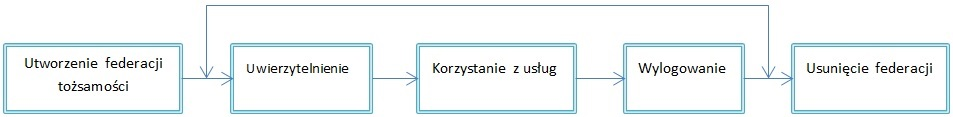
\includegraphics[width=15cm,height=2.5cm]{img/samlSSO.jpg}
				\caption{Schemat funkcjonowania mechanizmu jednokrotnego uwierzytelniania w SAML}
				\label{Schemat funkcjonowania mechanizmu jednokrotnego uwierzytelniania w SAML}
			\end{figure}

			Aby istniała możliwość korzystania z mechanizmu jednokrotnego uwierzytelniania konieczne jest utworzenie federacji pomiędzy tożsamościami jednostki. Po utworzeniu powiązań pomiędzy różnymi tożsamościami użytkownik po poprawnym uwierzytelnieniu względem jednej z usług może korzystać z innych sfederowanych serwisów. Wylogowanie się wykonane dla którejś z aplikacji powoduje zamknięcie dostępu do wszystkich sfederowanych usług. Procedura jednokrotnego uwierzytelniania może być wykorzystywana do momentu usunięcia federacji pomiędzy tożsamościami użytkownika.

		\paragraph{Przebieg procesu jednokrotnego uwierzytelniania w SAML}\mbox{}\\

			\begin{figure}[h]
				\centering
					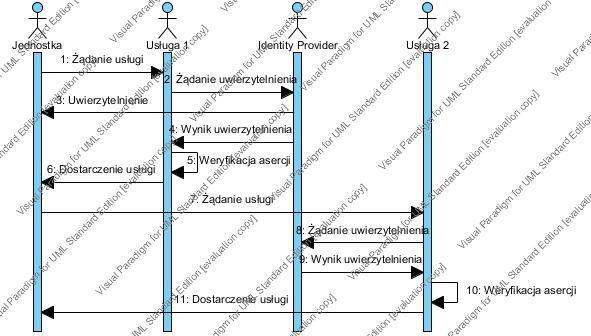
\includegraphics[width=15cm,height=10cm]{img/ssoSteps.jpg}
				\caption{Przebieg procesu jednokrotnego uwierzytelniania w SAML}
				\label{Przebieg procesu jednokrotnego uwierzytelniania w SAML}
			\end{figure}

			Usługa objęta mechanizmem jednokrotnego uwierzytelniania po otrzymaniu żądania udostępnienia swoich zasobów zleca modułowi "Identity Provider" przeprowadzenie procesu uwierzytelnienia klienta serwisu. Asercja będąca wynikiem procesu uwierzytelnienia zostaje przekazana do usługi zlecającej. Usługa dokonuje weryfikacji otrzymanej asercji i akceptuje lub odrzuca żądanie dostępu do zasobów. Gdy użytkownik chce skorzystać z usług innego serwisu sfederowanego z usługą, do której otrzymał dostęp, proces uwierzytelniania przebiega podobnie. Pomijany jest jednak krok ponownego uwierzytelniania użytkownika przez usługę "Identity Provider" - usługa ta zwraca do aplikacji żądającej uwierzytelniania asercję wygenerowaną na podstawie wcześniej wykonanego procesu uwierzytelniania.	
			
\subsection{OpenID}

OpenID

\subsection{Liberty Identity Web Services Framework}

	Identity Web Services Framework(ID-WSF) to zbiór specyfikacji definiujących mechanizmy dla zapewnienia bezpieczeństwa serwisów webowych, pomiędzy którymi istnieją relacje zaufania(federacje)\cite{Oracle10}. ID-WSF określa podejście do zarządzania tożsamościami, w którym tożsamości jednostek zarządzane są przez różnych dostawców usług połączonych relacją federacji. Usługi webowe mogą wymieniać między sobą dane osobowe swoich użytkowników w celu dostarczenia funkcjonalności żądanej przez klienta usługi. Przykładem sytuacji, gdzie może być zastosowany ten model jest usługa potrzebująca dostarczenia danych adresowych swojego użytkownika. W tym celu może skorzystać z zasobów innej usługi 
	dysponującej tymi danymi.

	Rysunek przedstawia przebieg procesu współdzielenia informacji w ID-WSF. Specyfikacja ID-WSF wprowadza dodatkowy element do architektury systemów zarządzania tożsamościami - "Discovery Service". Usługa "Discovery Service" pozwala dostawcom usług na wyszukiwanie innych serwisów dostarczających funkcjonalności pozwalających na realizacje żądań zadanych usłudze. Klient aplikacji decyduje o tym czy jego dane mogą być dostępne dla innych serwisów rejestrując usługę dostarczającą jego danych osobowych w rejestrze "Discovery Service" lub nie dokonując takiej rejestracji. Na przedstawionym schemacie żądana przez użytkownika usługa potrzebuje dodatkowych informacji - w tym celu w rejestrze usług szuka serwisu, który dostarcza potrzebnych informacji dla obsługiwanego użytkownika.

	\begin{figure}[h]
		\centering
			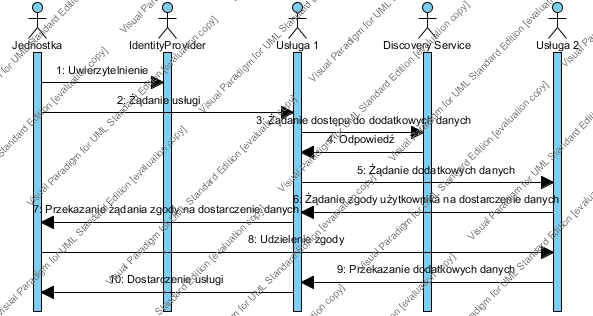
\includegraphics[width=15cm,height=9cm]{img/id-wsf.jpg}
		\caption{Przebieg procesu wykorzystywania informacji dzielonych w ID-WSF}
		\label{Przebieg procesu wykorzystywania informacji dzielonych w ID-WSF}
	\end{figure}

	ID-WSF definiuje również mechanizmy pozwalające na komunikację pomiędzy dostawcami usług i użytkownikiem w celu uzyskania zgody na przekazanie danych osobowych do innej aplikacji. Zaprezentowany diagram przedstawia ten proces. Usługa 2. po otrzymaniu żądania dostarczenia dodatkowych danych os Usługi 1. wymaga zgody użytkownika na udzielenie wymaganych informacji.
	
%---------------------------------------------------------------------------

\section{Przyklady frameworków zarzadzajacych autentykacja i autoryzacja uzytkowników}
\label{sec:frameworki}

Przyklady frameworków zarzadzajacych autentykacja i autoryzacja uzytkowników

%---------------------------------------------------------------------------

\chapter{Architektura proponowanego systemu}
\label{cha:architektura}

{\it

W ramach projektu przeprowadzono analizę wykorzystania mechanizmów wprowadzonych przez koncepcję systemów zarządzania tożsamościami dla różnych typów zastosowań. W tym celu zaproponowana została architektura dla przykładowych aplikacji. Jako specyfikację realizującą założenia systemów zarządzania tożsamościami wybrano standard SAML. Punktem wyjścia dla projektu było wdrożenie koncepcji jednokrotnego uwierzytelniania dla aplikacji webowych. Głównym elementem architektury systemu umożliwiającym tą funkcjonalność jest usługa ,,Identity Provider'' - potwierdzająca tożsamość użytkownika. Następnym krokiem było rozszerzenie mechanizmów uwierzytelniania opartych o protokół SAML na serwisy webowe. Zaproponowano architekturę systemu umożliwiającą uwierzytelnianie klientów usług webowych niezależnie od standardu dostarczania usług(np. SOAP lub REST) przy użyciu protokołu SAML. Głównym elementem architektury dla tego typu systemów jest usługa ,,Security Token Service'' - przydzielająca klientom tokeny potwierdzające ich tożsamość. 

Zastosowanie mechanizmów bezpieczeństwa protokołu SAML w architekturze zorientowanej na usługi zostało przeanalizowane na przykładzie prototypu systemu dokonywania zamówień w sklepie internetowym. Opracowano architekturę systemu składającego się z usług obsługujących różne etapy dokonywania zamówienia - sprawdzanie dostępności produktu, zlecenie przygotowania towaru do wydania, zlecenie dostawy, rejestracja transakcji w serwisie księgowym. Usługi  mogą być dostarczane przy zastosowaniu różnych standardów. Architektura systemu uwzględnia również wprowadzenie dodatkowej warstwy pośredniczącej w dostępie do serwisów - magistrali usług. Opracowano także model procesu biznesowego opisujący przebieg dokonywania zamówienia przy użyciu dostępnych usług. 

}

%---------------------------------------------------------------------------

\autsection{Podział na komponenty}{Krzysztof Wilaszek, Tomasz Wójcik}
\label{sec:komponenty}

	\subsection{Komponenty architektury aplikacji webowych z mechanizmem jednokrotnego uwierzytelniania}

		\begin{figure}[h]
			\centering
			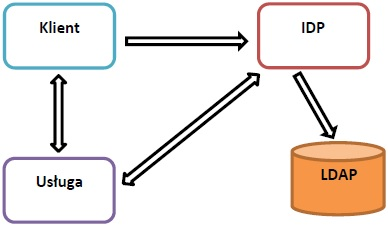
\includegraphics{img/samlWeb.jpg}
			\caption{Jednokrotne uwierzytelnianie aplikacji webowych w protokole SAML}
			\label{webSSO}
		\end{figure}

		Podstawowym elementem pozwalającym na realizację procedury jednokrotnego uwierzytelniania dla aplikacji webowych jest usługa ,,Identity Provider''. Usługa odpowiada za uwierzytelnianie klientów oraz dostarcza tożsamości użytkowników do zaufanych aplikacji. IdP wykorzystuje usługę katalogową LDAP jako bazę tożsamości. Dostawcy usług weryfikują tożsamość klienta żądającego dostępu do zasobów. Gdy konieczne jest uwierzytelniania - polegają na mechanizmach dostarczanych przez usługę IdP. Klient komunikuje się z usługą IdP w procesie uwierzytelniania przesyłając dane potwierdzające jego tożsamość.

	\subsection{Komponenty systemu uwierzytelniania klientów usług webowych w oparciu o standard SAML}

		\begin{figure}[h]
			\centering
			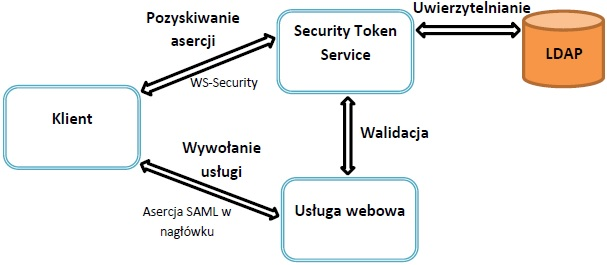
\includegraphics{img/samlWS.jpg}
			\caption{Uwierzytelnianie klienta serwisu webowego z wykorzystaniem SAML}
			\label{Uwierzytelnianie klienta serwisu webowego z wykorzystaniem SAML}
		\end{figure}

		Implementacja mechanizmu uwierzytelniania dla klientów usług webowych powinna korzystać z rozwiązań wprowadzonych przez standard WS-Trust. W skład infrastruktury systemu wchodzi usługa ,,Security Token Service'' odpowiedzialna za uwierzytelnianie użytkowników i generowanie asercji SAML. Serwis korzysta z bazy użytkowników udostępnianej np. przez usługę katalogową LDAP. Dzięki serwisowi STS klient pozyskuje token bezpieczeństwa - asercję SAML, która może być przekazywana do usługi, do której użytkownik chce uzyskać dostęp. Klient dokonuje procesu uwierzytelniania jednokrotnie - raz pozyskana asercja może zostać wykorzystana wielokrotnie dla różnych usług w celu potwierdzenia tożsamości klienta. Mechanizm uwierzytelniania klienta i pozyskiwania asercji korzysta ze specyfikacji WS-Security - użytkownik przekazuje do usługi STS swoje dane uwierzytelniające(identyfikator i hasło); gdy dane są poprawne usługa zwraca token bezpieczeństwa. Otrzymana asercja przekazywana jest w nagłówku SOAP lub HTTP(dla usług typu REST) do wywoływanych serwisów.

		Udostępniając usługi webowe, których zasoby powinny być chronione należy zagwarantować skuteczność kontroli dostępu do serwisu. Żaden nieuwierzytelniony lub nieuprawniony użytkownik nie powinien uzyskać praw dostępu do któregokolwiek z zasobów. Jednym z rozwiązań tego problemu jest centralizacja punktu uwierzytelniania i autoryzacji klientów serwisów - obsługa każdego otrzymanego żądanie użytkownika powinna rozpoczynać się od weryfikacji uprawnień klienta do pozyskiwanych zasobów. Rozwiązanie tego typu opisywane jest przez wzorzec ,,Message Interceptor Gateway''. 

		\begin{figure}[h]
			\centering
			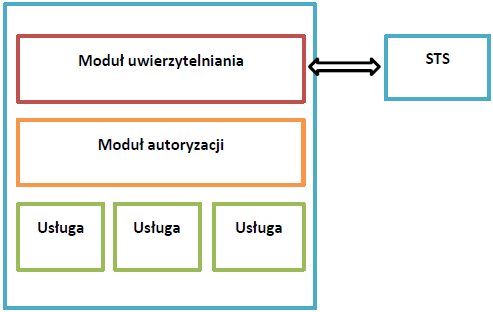
\includegraphics{img/interceptorGateway.png}
			\caption{Zastosowanie wzorca ,,Message Interceptor Gateway'' w procesie uwierzytelniania klienta serwisu webowego}
			\label{Zastosowanie wzorca ,,Message Interceptor Gateway'' w procesie uwierzytelniania klienta serwisu webowego}
		\end{figure}

		Zastosowanie wzorca wprowadza do systemu pojedynczy punkt weryfikacji uprawnień klienta do żądanych zasobów. Gwarantuje w ten sposób, że wszystkie zasoby w ramach jednej domeny będą odpowiednio chronione i każde żądanie użytkownika usługi przejdzie tą samą ścieżkę weryfikacji uprawnień przed przyznaniem prawa dostępu do funkcjonalności usługi. Obsługa żądań klientów rozpoczyna się od uwierzytelnienia klienta. Uwierzytelnianie odbywa się na podstawie asercji SAML przesyłanej w nagłówku wiadomości. Otrzymana asercja jest weryfikowana przy użyciu usługi ,,Security Token Service''. Dzięki asercji uznanej w procesie weryfikacji za poprawną możliwe jest dostęp do informacji o użytkowniku, np. jego nazwy oraz ról do jakich jest przypisany. Żądanie uwierzytelnionego użytkownika poddawane jest kolejnej weryfikacji w module autoryzacji. Moduł sprawdza, czy dany klient jest uprawniony do korzystania z usługi, do której chce uzyskać dostęp. W zaproponowanych rozwiązaniach wykorzystywany jest model autoryzacji RBAC(Role Based Access Control). Prawa dostępu weryfikowane są na podstawie przynależności użytkownika do określonej roli. Gdy moduł autoryzacji potwierdza uprawnienia klienta do usługi, udostępniane są mu zasoby serwisu.

	\subsection{Uwierzytelnianie klientów usług webowych przy użyciu asercji SAML w architekturze SOA}


		Zastosowanie koncepcji systemów zarządzania tożsamościami w architekturze zorientowanej na usługi przedstawione zostało na przykładzie prostego systemu obsługi zamówień sklepu internetowego. Opracowane zostały różne usługi realizujące poszczególne etapy dokonywania zamówienia. Serwisy zaimplementowane zostały przy użyciu różnych standardów dostarczania usług webowych(REST i SOAP). Wykorzystują schemat przebiegu procesu uwierzytelniania opisany w rozdziale ,,Komponenty systemu uwierzytelniania klientów usług webowych w oparciu o standard SAML'' niniejszej pracy. Proces uwierzytelniania oparty jest na mechanizmach opisanych standardem WS-Trust - wykorzystuje usługę ,,Security Token Service''. Proces zamówienia realizowany jest przez usługi odpowiedzialne za sprawdzanie stanu magazynu, zlecenie dostawy towaru, zlecenie wydania towaru  oraz rejestrację transakcji w serwisie księgowym. Usługi zlokalizowane są w różnych domenach. Uwierzytelnianie klientów usług opiera się na otrzymywanych asercjach SAML i wykorzystuje mechanizm weryfikacji tokenów bezpieczeństwa dostarczany przez usługę STS. 

	\subsection{Komponenty przykładowego systemu obsługi zamówień}	
		
		Stworzony system obsługi zleceń w sklepie internetowym stanowi „proof of concept” niniejszej pracy. Ponieważ dostarczane przez niego funkcje nie są szczególnie istotne z punktu widzenia analizy mechanizmów bezpieczeństwa, zostaną one opisane bez szczegółowej analizy. StoresStateService jest usługą udostępniającą informacje na temat stanu magazynowego sklepu. Przyjmuje ona nazwę oraz ilość egzemplarzy zamówionego produktu, a odpowiedź usługi zawiera lokację magazynu który posiada wymagany towar. WarehouseService rejestruje zamówienie w magazynie, zwracając potwierdzenie rejestracji. FinancialDepartmentService obsługuje system fakturowania, który zwraca identyfikator faktury. Ostatnim komponentem funkcjonalnym jest DeliveryService, który ma stanowić usługę dostarczaną przez zewnętrznego partnera biznesowego sklepu. Przyjmuje ona informacje o planowanej przesyłce, zwracając systemowi identyfikator przesyłki. 
		
		\begin{figure}[h]
			\centering
			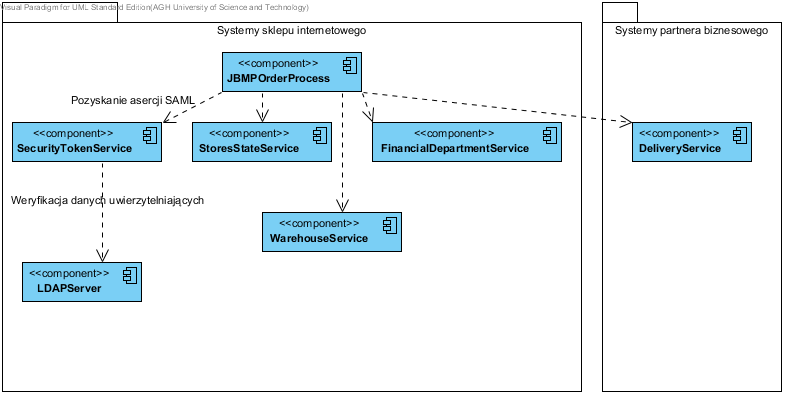
\includegraphics[width=\textwidth]{img/KomponentySystemu.png}
			\caption{Diagram komponentów przykładowego systemu obsługi zamówień}
			\label{Komponenty}
		\end{figure}	
		
%---------------------------------------------------------------------------

\autsection{Środowisko wdrożenia}{Tomasz Wójcik}
\label{sec:srodowiskoWdrozenia}

Jednym z wymagań pracy było uruchomienie stworzonego przykładowego systemu w środowisku chmury obliczeniowej. Ponieważ system ten był tworzony przy użyciu standardowych i dobrze wspieranych narzędzi(język programowania i biblioteki), naturalnym wyborem było wykorzystanie modelu Platform as a Service. Model pozwala na łatwiejsze wdrożenie aplikacji w porównaniu z IaaS, zachowując poziom elastyczności wymagany do zrealizowania postawionych wymagań projektowych, w przeciwieństwie do SaaS.

Użycie chmury obliczeniowej pozwala na łatwe przenoszenie poszczególnych komponentów pomiędzy serwerami i dynamiczne tworzenie domen bezpieczeństwa, pozwalając tym samym na przetestowanie zachowania systemu w środowisku wielodomenowym. Większość komponentów systemu może być uruchomiona wewnątrz jednego serwera aplikacji, w tej samej domenie bezpieczeństwa. Z punktu widzenia modelowania środowiska wielodomenowego, istotne jest jedynie to aby przynajmniej jeden komponent znalazł się w osobnej domenie.
Wykorzystane środowisko powinno udostępniać możliwość zewnętrznej komunikacji z wykorzystaniem protokołu HTTP, w celu udostępnienia usług sieciowych opartych o wzorzec REST i protokół SOAP. Chmura musi także umożliwiać komunikację pomiędzy usługą Security Token Service i serwerem LDAP. Z powodu ograniczeń technicznych serwer LDAP został uruchomiony na innym węźle niż tym na którym jest pracuje serwer aplikacji z systemem obsługi sklepu internetowego.
Końcową strukturę wdrożenia systemu obrazuje poniższy diagram.

		\begin{figure}[h]
			\centering
			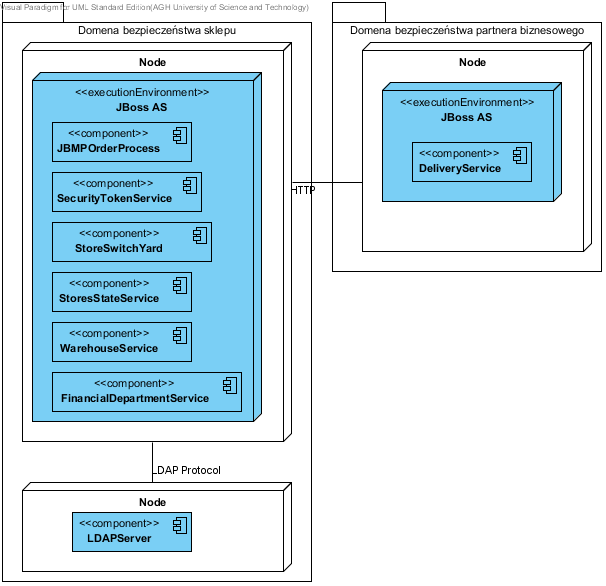
\includegraphics{img/DeploymentDiagram1.png}
			\caption{Diagram wdrożenia przykładowego systemu obsługi zamówień w środowisku chmury obliczeniowej}
			\label{DeploymentDiagram}
		\end{figure}

%---------------------------------------------------------------------------

\autsection{Zastosowane mechanizmy integracji}{Tomasz Wójcik}
\label{sec:integracja}

		\begin{figure}[h]
			\centering
			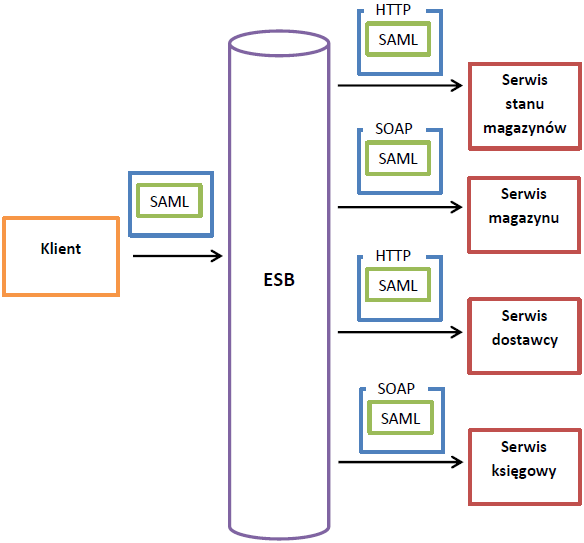
\includegraphics{img/esbAndSAML.png}
			\caption{Udział magistrali ESB w procesie wywołań usług z mechanizmami uwierzytelniania opartymi o SAML}
			\label{ESB i SAML}
		\end{figure}

		Do architektury proponowanego systemu wprowadzono dodatkową warstwę - magistralę usług(Enterprise Serial Bus). Magistrala usług pośredniczy w wywołaniach usług udostępnianych przez serwisy - otrzymuje wiadomości wraz z załączonymi tokenami bezpieczeństwa kierowane do przyłączonych serwisów. 
		
		Ponieważ klient serwisu odnosi się wyłącznie magistrali usług w celu skorzystania z usługi, nie musi on nic wiedzieć o rzeczywistym dostawcy usługi. Zapewnia to przezroczystość lokalizacji(ang. location transparency), która jest szczególnie istotna w środowisku chmury obliczeniowej, w którym rzeczywista lokacja usługi może dynamicznie się zmieniać. Podejście to ułatwia także zapewnienie skalowalności poprzez umożliwienie zwielokrotnienia instancji dostawców usług.
		Jednym z głównych cech większości rozwiązań typu ESB jest pośredniczenie w transformacji wiadomości i konwersji protokołów pomiędzy nadawcą a odbiorcą wiadomości. Magistrala dostosowuje otrzymywane wiadomości do formatu wykorzystywanego przez daną usługę. W przypadku stworzonego przykładowego systemu obsługi zamówień, magistrala udostępnia zasoby REST stanowiące interfejs kliencki do usług realizowanych przez serwisy uruchomione w systemie.
		
		Zadania magistrali usług w kontekście obsługi tokenów bezpieczeństwa są ograniczone. Moduł ESB nie dokonuje analizy ani przetwarzania otrzymywanych asercji SAML. Jedynym zadaniem magistrali w procesie obsługi tokenów bezpieczeństwa jest dołączenie tokenu do nagłówka odpowiedniego typu dla danego formatu wiadomości akceptowanych przez usługę.
		Strukturę komponentów po wprowadzeniu magistrali usług przedstawia poniższy diagram.

		\begin{figure}[h]
			\centering
			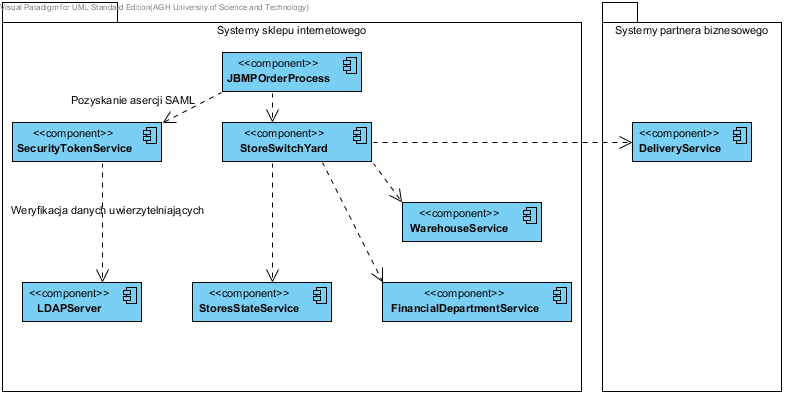
\includegraphics[width=\textwidth]{img/KomponentySystemuESB.png}
			\caption{Diagram komponentów przykładowego systemu obsługi zamówień z wykorzystaniem ESB}
			\label{KomponentyESB}
		\end{figure}
		
%---------------------------------------------------------------------------

\chapter{Stos technologiczny}
\label{cha:stosTechnologiczny}

{\it

W celu realizacji wymagań stawianych opracowywanym aplikacjom wykorzystane zostały różne technologie umożliwiające implementację określonych aspektów dostarczanych funkcjonalności.

Wdrożenie zabezpieczeń dostępu do aplikacji oparte o zostało na mechanizmach definiowanych przez serwer aplikacyjny JBoss. Serwer JBoss pozwala konfigurować systemy i domeny bezpieczeństwa oraz stosowane w ich obrębie mechanizmy uwierzytelniania i autoryzacji użytkowników usług. Proces uwierzytelniania klientów aplikacji wykorzystuje mechanizmy implementowane poprzez protokół LDAP. 

Przykładowe aplikację wykorzystują realizację standardu SAML - projekt Picketlink. Picketlink definiuje model tożsamości wykorzystywana w procesie uwierzytelniania, pozwala na stosowanie standardu - WS-Trust w celu obsługi funkcjonalności federacji tożsamości. Dostarcza implementację modułów ,,Identity Provider'' oraz ,,Security Token Service''. 

}

%---------------------------------------------------------------------------

\section{Mechanizmy bezpieczenstwa platformy Java SE}
\label{sec:javaSE}

Mechanizmy bezpieczenstwa platformy Java SE

%---------------------------------------------------------------------------


\section{Mechanizmy bezpieczenstwa platformy Java EE}
\label{sec:javaEE}

Mechanizmy bezpieczenstwa platformy Java EE

%---------------------------------------------------------------------------

\autsection{Protokół LDAP}{Krzysztof Wilaszek}
\label{sec:ldap}

	LDAP(Lightweight Directory Access Protocol) jest protokołem definiującym metody, dzięki którym możliwy jest dostęp do danych zawartych w katalogach\cite{ZyTrax13}. Opisuje sposób reprezentacji danych w usłudze katalogowej oraz definiuje metody ładowania i eksportowania danych. Bazuje na standardzie X.500.

	\subsection{Model działania protokołu LDAP}

		\begin{figure}[h]
			\centering
			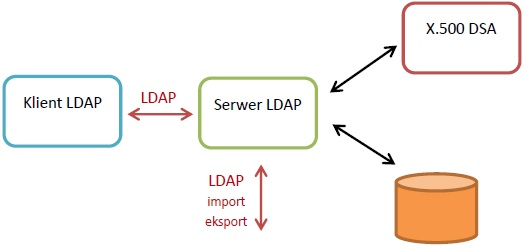
\includegraphics{img/ldap.jpg}
			\caption{Schemat funkcjonowania protokolu  LDAP}
			\label{Schemat funkcjonowania protokolu  LDAP}
		\end{figure}

		Protokół LDAP definiuje sposób dostępu do zasobów, nie określa natomiast sposób przechowywania danych. Jednym z wariantów jest przechowywanie informacji w bazie danych. Użytkownik komunikujący się z serwerem LDAP nie wie skąd pochodzą dane, które otrzymuje. Protokół LDAP definiuje również metody ładowania danych do usługi katalogowej oraz eksportowania danych z usługi przy użyciu formatu LDIF. Protokół LDAP opisuje operacje jakie mogą być wykonywane na modelu danych(np. modyfikowanie, usuwanie, odczyt).

	\subsection{Reprezentacja danych w protokole LDAP}

		Dane w protokole LDAP reprezentowane są w postaci hierarchii obiektów\cite{ZyTrax13}. Obiekty tworzą strukturę drzewa nazywanego drzewem DIT(Data Information Tree). Wierzchołek drzewa to element ,,root''. Każdy element drzewa składa się z co najmniej jednej klasy obiektów. Klasa obiektów to zbiór atrybutów przypisanych do obiektu. Każdy atrybut posiada nazwę i najczęściej ma przypisaną wartość. Klasa obiektu określa czy nadanie wartości danego atrybutu jest obowiązkowe czy opcjonalne. Obiekty identyfikowane są poprzez swoje położenie w drzewie - ścieżkę określającą elementy drzewa na drodze do obiektu. Identyfikator obiektu nazywany jest elementem Distinguished Name(DN).

	\subsection{Uwierzytelnianie przy użyciu protokołu LDAP}

		Usługa katalogowa LDAP może być wykorzystywana jako baza informacji o użytkownikach  i serwis uwierzytelniający. LDAP pozwala również na przechowywanie informacji o rolach użytkowników. 

		Proces uwierzytelniania przy użyciu protokołu LDAP rozpoczyna się od pozyskania mapowania pomiędzy identyfikatorem użytkownika w systemie a elementem DN usługi katalogowej. Następnie wykonywana jest operacja uwierzytelniania w serwerze LDAP - ,,bind''. Aby wykonać operację ,,bind'' konieczne jest przesłanie nazwy DN i hasła użytkownika.  Innym sposobem uwierzytelnienia użytkownika może być porównanie przedstawionego przez niego hasła z hasłem przechowywanym przez usługę katalogową. Dla uwierzytelnionego użytkownika możliwe jest pobranie listy jego ról i uprawnień.

%---------------------------------------------------------------------------

\autsection{Mechanizmy bezpieczeństwa serwera aplikacyjnego JBoss}{Krzysztof Wilaszek}
\label{sec:jboss}

	Mechanizmy bezpieczeństwa serwera aplikacyjnego JBoss w wersji 7 oparte są o framework PicketBox. PicketBox dostarcza podstawowych funkcjonalności zapewnienia bezpieczeństwa dostępu do zasobów, takich jak uwierzytelnianie, autoryzacja, audyty systemu oraz mapowanie ról i danych uwierzytelniających. 

	\subsection{Podsystemy bezpieczeństwa serwera aplikacyjnego JBoss}

		Usługi bezpieczeństwa dostarczane przez Picketbox są dostępne dla serwera aplikacyjnego poprzez podsystem bezpieczeństwa(ang. Security Subsystem).  Każdemu żądaniu klienta przypisywany jest kontekst bezpieczeństwa dostępny dla podsystemu bezpieczeństwa\cite{Lofthouse12}. 

		Kontekst bezpieczeństwa udostępnia komponenty skonfigurowane dla domeny bezpieczeństwa. Możliwe komponenty to:

		\begin{itemize}
			\item Authentication Manager - dokonuje uwierzytelniania użytkowników na podstawie otrzymanych danych uwierzytelniających przy użyciu modułów logowania zdefiniowanych dla wykorzystywanej domeny bezpieczeństwa;
			\item Authorization Manager - dostarcza informacji o rolach przypisanych użytkownikowi oraz dokonuje autoryzacji dostępu do zasobów dla uwierzytelnionych użytkowników;
			\item Audit Manager - pozwala na logowanie zdarzeń zachodzących w systemie zapewnienia bezpeiczeństwa dostępu do aplikacji;
			\item Mapping Manager - pozwala na przypisywanie uwierzytelnionemu użytkownikowi dodatkowych uprawnień, ról lub atrybutów.
		\end{itemize}

		Korzystania z podsystemów bezpieczeństwa możliwe jest dzięki dodaniu rozszerzenia:
		\lstset{language=XML}
		\begin{lstlisting}
	<extension module="org.jboss.as.security"/>
		\end{lstlisting}
		w pliku konfiguracyjnym serwera.

		Podsystem bezpieczeństwa serwera aplikacyjnego JBoss udostępnia konfigurację następujących własności:

		\begin{itemize}
			\item security-management - pozwala nadpisywać domyślne parametry modułu PicketBox takie jak implementacje klas zarządców dla procesów uwierzytelniania, autoryzacji, audytów, mapowania danych tożsamości oraz tworzenia relacji zaufania.
			\item security-domains - pozwala na konfiguracje domen bezpieczeństwa
			\item security-properties - pozwala definiować dodatkowe własności wymagane przez podsystem bezpieczeństwa.
		\end{itemize}

	\subsection{Domena bezpieczeństwa serwera aplikacyjnego JBoss}

		W ramach podsystemu bezpieczeństwa możliwa jest definicja domen bezpieczeństwa. Domena bezpieczeństwa opisuje mechanizmy zabezpieczeń dostępu do aplikacji wykorzystywane przez grupę usług przypisanych do tej domeny.

		Podstawowym zadaniem domeny bezpieczeństwa jest przeprowadzanie procesu uwierzytelniania klientów aplikacji. W tym celu do domeny przypisane są moduły logowania(ang. ,,Login Module'') wykorzystywane do uwierzytelniania użytkowników. Konfigurując moduł logowania należy wybrać klasę definiującą sposób i przebieg uwierzytelniania użytkownika. Domyślnie dostępne są implementacje pozwalające na uwierzytelnianie np. w oparciu o certyfikaty, bazę danych z użytkownikami i hasłami, protokół LDAP, protokół Kerberos lub prosty plik z użytkownikami i hasłami.

		Możliwe jest również oparcie mechanizmów uwierzytelniania o specyfikację JASPI(Java Authentication Service Provider Interface for Containers). JASPI definiuje standardowy interfejs dla dostawców usług, przy pomocy którego dla kontenera aplikacji Java EE możliwe jest uwierzytelnianie na podstawie danych bezpieczeństwa przesyłanych na poziomie wiadomości. Specyfikacja określa mechanizmy strony klienckiej oraz serwerowej. Serwer ma możliwość weryfikacji tokenów bezpieczeństwa lub podpisów przychodzących wiadomości i pozyskania opisu uprawnień użytkownika lub asercji. Strona kliencka może dodawać do wysyłanych wiadomości token bezpieczeństwa lub podpis cyfrowy. 

		Inny ważnym mechanizmem definiowanym na poziomie domeny bezpieczeństwa jest autoryzacja klientów aplikacji. Domyślnie realizowanym podejściem w procesie autoryzacji jest RBAC(Role Based Access Control). Metoda ta przydziela lub odmawia prawa dostępu do zasobów w oparciu o przynależność użytkownika do określonej grupy. Możliwe jest również użycie innych metod autoryzacji, np. JACC(Java Authorization Contract for Containers) lub XACML (eXtensible Access Control Markup Language). 

		Definicja domeny bezpieczeństwa obejmuje również:

		\begin{itemize}
			\item mapowania ról, uprawnień, danych uwierzytelniających i atrybutów; 
			\item konfigurację mechanizmu audytów operacji w domenie bezpieczeństwa
			\item konfigurację repozytorium certyfikatów bezpieczeństwa wykorzystywanych przez kontekst SSL lub przez procesy pozyskiwania i magazynowania certyfikatów.
		\end{itemize}
		
%---------------------------------------------------------------------------

\section{Security Assertion Markup Language}
\label{sec:saml}

Security Assertion Markup Language

%---------------------------------------------------------------------------

\autsection{Picketlink}{Krzysztof Wilaszek}
\label{sec:picketlink}

Picketlink jest projektem dostarczającym implementacji założeń systemów zarządzania tożsamościami dla aplikacji Java. Picketlink definiuje model tożsamości wykorzystywanych w operacjach systemów IdM. Pozwala na zarządzanie informacjami o użytkownikach, grupach i rolach oraz ich atrybutach. Umożliwia wykorzystanie różnych sposobów przechowywania tożsamości, np. bazy danych lub usługi katalogowej LDAP. Projekt Picketlink umożliwia korzystanie z federacji tożsamości - wspiera specyfikacje SAML, OpenID oraz WS-Trust\cite{PicketLink13}.

Picketlink dostarcza wsparcie dla profili specyfikacji SAML umożliwiających jednokrotne uwierzytelnianie aplikacji webowych oraz globalne wylogowanie. Określa również mapowania dla protokołu HTTP przy użyciu komunikatów POST i Redirect. 

Picketlink implementuje mechanizmy pozwalające na tworzenie usługi ,,Identity Provider''. Dostarcza narzędzi konfiguracji usługi, uwierzytelniania a także implementację operacji obsługi przechowywania tożsamości. W ramach konfiguracji możliwe jest między innymi określenie zaufanych hostów dla usługi IdP, ustawienie cyfrowego podpisu dla wiadomości oraz szyfrowanie komunikatów. Usługa ,,Identity Provider'' w procesie uwierzytelniania może korzystać z mechanizmu domen bezpieczeństwa serwera aplikacyjnego JBoss. Dostawcy usług korzystają z serwisu IdP w pozyskując asercje opisujące użytkowników. Picketlink umożliwia taką konfigurację usług aby ich mechanizmy uwierzytelniania korzystały z usługi IdP.

Narzędzia Picketlink dostarczają implementacji specyfikacji WS-Trust - za operacje zarządzania asercjami SAML(tworzenie, odnawianie, anulowanie i walidację) odpowiada usługa ,,Security Token Service''. Moduł Picketlink zawiera implementację usługi STS oraz pozwala konfigurować parametry takie jak szyfrowanie tokenu bezpieczeństwa i wymóg dołączania cyfrowego podpisu dla tokenów. Moduł implementuje narzędzia przechwytywania wywołań usług webowych i weryfikacji wymaganych asercji uprawniających do dostępu do zasobów. 

%---------------------------------------------------------------------------

\section{Business Process Management}
\label{sec:bpm}

Business Process Management

%---------------------------------------------------------------------------

\section{Enterprise Service Bus}
\label{sec:esb}

Enterprise Service Bus

%---------------------------------------------------------------------------

\section{OpenShift}
\label{sec:openShift}

OpenShift

%---------------------------------------------------------------------------
\chapter{Opis implementacji}
\label{cha:implementacja}

{\it

Zgodnie z założeniami architektury dla proponowanych rozwiązań i przy wykorzystaniu technologii opisanych we wcześniejszych rozdziałach niniejszej pracy zaimplementowano przykładowe aplikacje prezentujące wykorzystanie koncepcji systemów zarządzania tożsamościami przy użyciu specyfikacji SAML. Najbardziej podstawowym spośród zrealizowanych scenariuszy było zastosowanie asercji SAML w procesie uwierzytelniania klientów aplikacji webowych - udostępnianych poprzez przeglądarkę internetową. Główną rolę w proponowanym rozwiązaniu odgrywa moduł ,,Identity Provider'' odpowiedzialny za procesy uwierzytelniania użytkowników aplikacji.

Implementacja mechanizmów jednokrotnego uwierzytelniania klientów aplikacji webowych przy użyciu standardu SAML była punktem wyjścia dla wdrożenia koncepcji zarządzania tożsamościami dla systemów w architekturze zorientowanej na usługi. Opracowane zostały aplikacje wykorzystujące standard SAML w procesie uwierzytelniania klientów usług webowych(przy użyciu standardów SOAP i REST). Realizacja tych mechanizmów wykorzystuje model architektury uwierzytelniania klientów serwisów webowych opisany w niniejszej  pracy. Zaimplementowano usługi realizujące poszczególne etapy procesu dokonywania zamówienia w sklepie internetowym. Usługi zostały wykorzystane jako przykład zastosowania mechanizmów SAML w architekturze SOA. Wprowadzona została warstwa pośrednicząca pomiędzy wywołaniami klienta a dostarczanymi serwisami - magistrala usług ESB. Zastosowano również narzędzia modelowania procesów biznesowych w celu skomponowania procesu realizacji zamówienia przy użyciu dostępnych usług z wykorzystaniem uwierzytelniania opartego o tokeny bezpieczeństwa SAML. Aplikacja została wdrożona w środowisku chmury obliczeniowej - OpenShift.

}

%---------------------------------------------------------------------------

\autsection{Implementacja mechanizmu jednokrotnego uwierzytelniania klientów aplikacji webowych}{Krzysztof Wilaszek}

	Przy pomocy mechanizmów udostępnianych przez narzędzia \textit{Picketlink} zaimplementowana została usługa ,,Identity Provider'' odpowiedzialna za uwierzytelnianie użytkowników systemu. Stosując usługę IdP możliwe jest jednokrotne uwierzytelnianie klientów aplikacji webowych. Zaimplementowane zostały również aplikacje wykorzystujące usługę IdP jako mechanizm uwierzytelniania klientów żądających dostępu do zasobów aplikacji.

	\begin{figure}[h]
		\centering
		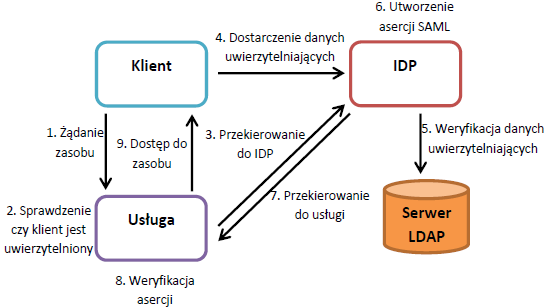
\includegraphics{img/samlWebSSO.png}
		\caption{Przebieg procesu jednokrotnego uwierzytelniania klientów aplikacji webowych w protokole SAML}
		\label{samlSSOSteps}
	\end{figure}
		
	Kiedy użytkownik chce uzyskać dostęp do zasobów, usługa sprawdza czy klient jest uwierzytelniony. Jeśli nie jest uwierzytelniony następuje przekierowanie do usługi ,,Identity Provider''. Klient podaje swoje dane uwierzytelniające a IdP weryfikuje ich poprawność. Gdy dane są prawidłowe generowana jest asercja SAML i następuje przekierowanie do usługi. Usługa weryfikuje otrzymaną asercję i przydziela lub odmawia prawa dostępu do zasobu. Gdy klient chce uzyskać dostęp do zasobów innej aplikacji nie musi ponownie podawać swoich danych uwierzytelniających, usługa IdP nie dokonuje ponownie procesu uwierzytelniania w usłudze katalogowej LDAP.
	
	W oparciu o przedstawiony schemat zaimplementowane zostały przykładowe usługi dostarczające funkcjonalności realizacji poszczególnych etapów  zamówienia w sklepie internetowym. Opracowano serwisy umożliwiające sprawdzanie stanu magazynu, zlecenie dostawy, obsługę wydawania towarów oraz rejestrację transakcji w serwisie finansowym. Zaimplementowane usługi wykorzystują różne standardy dostarczania usług sieciowych - REST lub SOAP. 

%---------------------------------------------------------------------------

\autsection{Implementacja mechanizmu uwierzytelniania klientów usług webowych}{Krzysztof Wilaszek}

	Implementacja mechanizmów uwierzytelniania klientów usług sieciowych oparta jest na modelu systemu prezentowanym w rozdziale opisującym architekturę dla proponowanych rozwiązań. Zaimplementowane zostały usługi różnych standardów(SOAP i REST) wykorzystujące asercje SAML w procesie uwierzytelniania swoich klientów. Zgodnie z zaproponowanym modelem w systemie istnieje usługa ,,Security Token Service'' odpowiedzialna za przydzielanie tokenów bezpieczeństwa użytkownikom. Otrzymany token bezpieczeństwa dołączany jest do żądania przesyłanego do serwisu. Przed przyznaniem dostępu do żądanych funkcjonalności treść wiadomości przechwytywana jest przez mechanizm specyficzny dla danego typu serwisu. Dla usług opartych o standard SOAP są to mechanizmy typu \textit{,,Handler''}. Dla usług dostarczanych w standardzie REST jest to mechanizm typu \textit{,,Interceptor''} dostarczany przez bibliotekę RESTEasy - implementację technologi dostarczania usług sieciowych typu REST. Mechanizmy dostarczane przez RESTEasy grupują \textit{interceptory} na klasy o różnych priorytetach. Klasą o najwyższym priorytecie(której metody wykonywane są najwcześniej) są \textit{interceptory} bezpieczeństwa. Dzięki zastosowaniu tej grupy możliwa jest realizacja wymagania przeprowadzenia procesu uwierzytelniania klienta na samym początku przetwarzania jego żądania i uniemożliwienia dostępu do jakichkolwiek zasobów dla nieuwierzytelnionych użytkowników.

	\begin{figure}[h]
		\centering
		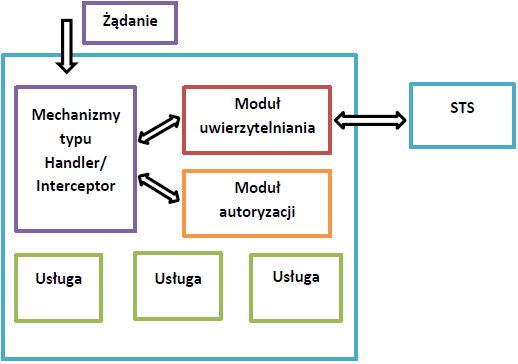
\includegraphics{img/interceptorGatewayImplementation.png}
		\caption{Uwierzytelnianie klientów usług webowych przy użyciu asercji SAML}
		\label{interceptorGatewayImplementation}
	\end{figure}

	Przechwycona wiadomość poddawana jest procesom wstępnej analizy. Między innymi wydobywana jest asercja SAML i przy jej wykorzystaniu wykonywany jest proces uwierzytelniania użytkownika. W trakcie uwierzytelniania asercja przesyłana jest do usługi ,,Security Token Service'' w celu weryfikacji jej poprawności. Po poprawnym uwierzytelnieniu klienta usługi następuje proces autoryzacji - dostęp do zasobów przyznawany jest na podstawie wiadomości o przynależności do określonych grup użytkowników. Wiadomość o grupach klienta zawarta jest w asercji SAML.

	W oparciu o przedstawiony schemat zaimplementowane zostały przykładowe usługi dostarczające funkcjonalności poszczególnych etapów realizacji zamówienia w sklepie internetowym. Opracowano serwisy umożliwiające sprawdzanie stanu magazynu, zlecenie dostawy, obsługę wydawania towarów oraz rejestrację transakcji w serwisie finansowym. Zaimplementowane usługi wykorzystują różne standardy dostarczania usług sieciowych - REST lub SOAP. 
	

%---------------------------------------------------------------------------

\autsection{Implementacja mechanizmów bezpieczeństwa w architekturze zorientowanej na usługi}{Krzysztof Wilaszek}

\subsection{Implementacja modułu magistrali usług}

	Implementacja mechanizmu magistrali usług wykorzystuje framework ,,Switchyard''. Przy pomocy narzędzi ,,Switchyard'' konfigurowane są punkty końcowe, na których nasłuchiwane są nadchodzące komunikaty. Przetwarzanie otrzymanych wiadomości realizowane jest przy użyciu narzędzi ,,Camel''. ,,Camel'' dostarcza mechanizmy zarządzania ścieżką jaką kierowane są wiadomości oraz implementuje wzorce EIP(\textit{Enterprise Integration Patterns}). Implementacja mechanizmu przetwarzania wiadomości magistrali usług przedstawiona zostanie na przykładzie wywołań serwisów webowych dostarczanych przy użyciu technologii SOAP(rysunek \textit{,,Implementacja przetwarzania wiadomości przez magistralę usług''}).

	\begin{figure}[h]
		\centering
		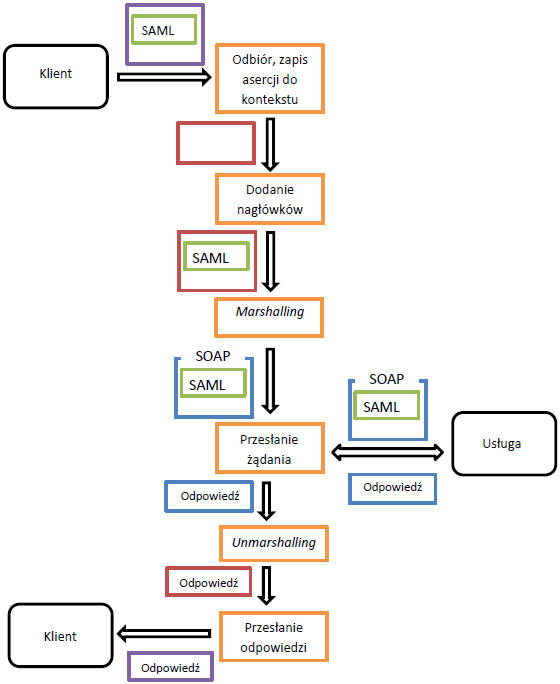
\includegraphics{img/esbRoute.png}
		\caption{Implementacja przetwarzania wiadomości przez magistralę usług}
		\label{ESB route}
	\end{figure}

	Klient wywołując usługi przesyła komunikaty określonego formatu - korzystając z określonej metody dostępu do zdalnych serwisów. Moduł magistrali usług otrzymuje komunikat żądania usługi. Do komunikatu dołączony jest nagłówek, w którym przesyłany jest token bezpieczeństwa - asercja SAML. Otrzymany komunikat przekształcany jest do formatu wykorzystywanego wewnętrznie przez moduł przetwarzania wiadomości a informacje zawarte w nagłówku(w tym asercja SAML) zapisywane są w kontekście przetwarzania. Do budowanej wiadomości dodawane są nagłówki(informacje kontekstowe) - dzięki czemu dołączany jest token bezpieczeństwa. Następnie dokonywany jest proces \textit{marshallowania} zbudowanej wiadomości - asercja SAML wpisywana jest do nagłówka(np. SOAP) utworzonego komunikatu. Po serializacji informacji następuje wywołanie usługi korzystające ze zbudowanej wiadomości. Usługa przeprowadza procesy uwierzytelniania klienta i autoryzacji dostępu do zasobów. Po poprawnym przebiegu tych kroków zwracana jest odpowiedź serwisu. Odpowiedź jest \textit{unmarshallowana} i przesyłana do klienta w formacie zgodnym z metodą wywołania usługi.

	Dostęp do serwisów obsługujących poszczególne etapy realizacji zamówienia w przykładowym systemie sklepu internetowego odbywa się za pośrednictwem mechanizmu magistrali usług zaimplementowanego zgodnie z opisanym schematem. 
	
	\subsection{Zastosowanie narzędzi modelowania procesów biznesowych}

	Serwisy udostępniane poprzez moduł magistrali usług dostarczają funkcjonalności realizujących poszczególne etapy przetwarzania zamówienia w sklepie internetowym. Przy użyciu narzędzi zarządzania procesami biznesowymi \textit{jBPM} opracowany został model procesu biznesowego wykorzystujący usługi udostępnianie poprzez moduł magistrali \textit{ESB} w celu realizacji zamówienia w sklepie internetowym. Model zakłada zastosowanie mechanizmów jednokrotnego uwierzytelniania z użyciem standardu \textit{SAML} w procesie uzyskiwania dostępu do usług poszczególnych serwisów realizujących kolejne etapy zamówienia. 

		\begin{figure}[h]
			\centering
			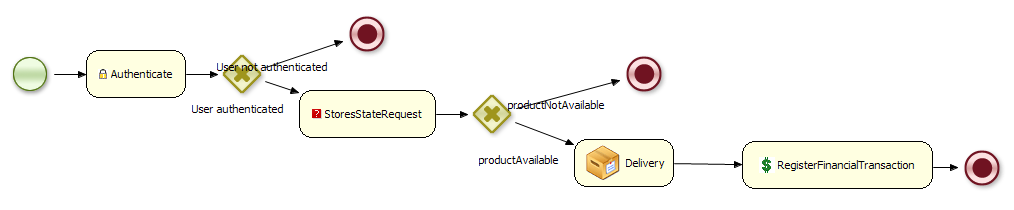
\includegraphics[width=18cm,height=4cm]{img/jbpm_order_process.png}
			\caption{Zastosowanie narzędzi modelowania procesów biznesowych z wykorzystaniem mechanizmów jednokrotnego uwierzytelniania}
			\label{jBPM process}
		\end{figure}

	Punktem wejściowym przedstawionego modelu procesu biznesowego jest uwierzytelnienie klienta serwisu. W wyniku poprawnego przebiegu uwierzytelniania klient otrzymuje token bezpieczeństwa - asercję SAML. Uzyskana asercja wykorzystywana jest w procesie przyznawania dostępu do usług konkretnych serwisów odpowiadających za poszczególne etapy realizacji zamówienia. Zastosowanie asercji SAML i wykorzystanie modelu opisanego przez specyfikację WS-Trust pozwala na osiągnięcie funkcjonalności jednokrotnego uwierzytelniania klienta procesu biznesowego - token bezpieczeństwa pozyskany na etapie uwierzytelniania identyfikuje klienta aplikacji podczas korzystania z usług poszczególnych serwisów wchodzących w skład procesu.
%---------------------------------------------------------------------------

\autsection{Wdrożenie systemu w środowisku OpenShift}{Tomasz Wójcik}
Wdrożenie systemu w środowisku OpenShift


\chapter{Analiza zastosowań tworzonego systemu}
\label{cha:zastosowania}

{\it

Niniejszy rozdział przedstawia możliwości zastosowania proponowanych rozwiązań w rzeczywistych systemach o architekturze SOA oraz wynikające z tego korzyści. Wykorzystanie mechanizmów systemów zarządzania tożsamościami pozwala zapewnić bezpieczeństwo aplikacji o architekturze zorientowanej na usługi. Zastosowany standard SAML i definiowane przy jego użyciu mechanizmy stanowią rozwiązanie dobrze dopasowane do specyfiki systemów o architekturze SOA. Elastyczność i skalowalność proponowanego podejścia sprawiają, że możliwe jest jego efektywne wdrożenie w rzeczywistym środowisku systemu bazującego na architekturze SOA.

Druga część rozdziału podsumowuje przydatność głównych rozwiązań technologicznych zastosowanych w projekcie w tworzeniu systemów o charakterze SOA.

Rozdział opisuje również potencjalne ulepszenia proponowanego rozwiązania. Zwiększenie poziomu bezpieczeństwa i rozszerzenie funkcjonalności systemu mogłoby być możliwe np. dzięki: wprowadzeniu wielu usług uwierzytelniających STS powiązanych relacją zaufania, zastosowaniu szyfrowania i podpisów na poziomie fragmentów przesyłanych wiadomości oraz możliwości definiowania parametrów bezpieczeństwa przy użyciu polityk.

}

%---------------------------------------------------------------------------

\section{Możliwości wykorzystania środowiska w praktyce}
\label{sec:wykorzystanieWPraktyce}

	System powstały w wyniku wykonanych prac projektowych stanowi przykład wykorzystania podejścia opartego o zarządzanie tożsamościami jako metody zapewnienia bezpieczeństwa dostępu do aplikacji w architekturze SOA. Przygotowana implementacja dowodzi, że  istnieje możliwość oparcia funkcjonowania mechanizmów bezpieczeństwa aplikacji w architekturze SOA na rozwiązaniach dostarczanych przez systemy zarządzania tożsamościami. 

	Wynikiem prac implementacyjnych jest system wykorzystujący standard SAML jako realizację założeń systemów zarządzania tożsamościami. Przygotowany system dostarcza przykładów zastosowania specyfikacji SAML jako metody uwierzytelniania klientów usług sieciowych. Wykorzystanie  SAML w procesie uwierzytelniania umożliwia implementację mechanizmów bezpieczeństwa dla usług opartych o różne standardy dostarczania usług sieciowych(np. SOAP i REST). Do architektury przykładowego systemu wprowadzono również moduł magistrali usług - ESB, będący charakterystycznym elementem systemów opartych o architekturę SOA. Zaproponowana implementacja modułu magistrali usług dostarcza funkcjonalności przetwarzania wiadomości z dołączonymi tokenami bezpieczeństwa - asercjami języka SAML. Dzięki zastosowaniu mechanizmów bezpieczeństwa bazujących na specyfikacji SAML możliwe było osiągnięcie funkcjonalności jednokrotnego uwierzytelniania klienta dla różnych usług systemu o architekturze typu SOA. Mechanizm jednokrotnego uwierzytelniania może być wykorzystany podczas budowania procesu biznesowego odwołującego się do różnych usług sieciowych.

	Zastosowanie mechanizmów systemów zarządzania tożsamościami w kontekście aplikacji w architekturze SOA jest rozwiązaniem posiadającym wiele zalet. Może stanowić sposób standaryzacji implementacji mechanizmów zapewniania bezpieczeństwa aplikacji. Opiera się na oddelegowaniu odpowiedzialności związanych z bezpieczeństwem aplikacji do specjalizowanych usług. Dzięki zastosowaniu standardu SAML możliwe jest tworzenie relacji zaufania pomiędzy różnymi usługami uwierzytelniania i autoryzacji. Dzięki temu klient aplikacji może w transparentny dla siebie sposób korzystać z usług w obrębie różnych domen bezpieczeństwa. Zastosowanie zarządzania tożsamościami jest podejściem elastycznym, skalowalnym, umożliwiającym efektywne rozszerzanie na kolejne elementy infrastruktury systemu. Oddelegowanie odpowiedzialności związanych z uwierzytelnianiem i autoryzacją do odrębnej, specjalizowanej usługi zwiększa poziom bezpieczeństwa systemu. Wykorzystanie specyfikacji SAML umożliwia realizację procesu jednokrotnego uwierzytelniania klienta korzystającego z wielu usług sieciowych.

	Proces zapewnienia bezpieczeństwa dostępu do systemu opartego o architekturę SOA może być realizowany z wykorzystaniem mechanizmów zarządzania tożsamościami. Zaproponowane rozwiązanie wykorzystujące standard SAML jest podejściem dobrze dopasowanym do specyfiki i wymagań systemów o architekturze SOA.

%---------------------------------------------------------------------------

\section{Użyteczność zastosowanych technologii w systemach udostępniania usług}
\label{sec:uzytecznosc}

Przy pomocy wymienionych w tekście pracy technologii, udało się stworzyć prosty system obsługi zleceń w sklepie internetowym. Sam ten fakt dowodzi już, że wybrane technologie można z powodzeniem zastosować w aplikacjach o charakterze SOA. Jednak poszczególne elementy budujące system mogą się od siebie znacznie różnić pod względem użyteczności.

Java jest prawdopodobnie najpopularniejszym językiem służącym do tworzenia systemów zorientowanych na usługi. Pewne cechy języka zapewniały mu pozycję lidera w klasie aplikacji typu enterprise jeszcze przed spopularyzowaniem konceptu SOA. Sam język jest stosunkowo łatwy w nauce i popularny. Zapewnia wsteczną kompatybilność, bardzo ważną dla systemów korporacyjnych, które często cechuje długi cykl życia. Posiada bardzo dobrą dokumentację i rozbudowaną bibliotekę standardową, umożliwiającą przetwarzanie wiadomości w formacie XML(JAXP, JAXB). Java Enterprise Edition definiuje dodatkowo wiele API szczególnie przydatnych w aplikacjach SOA, takich jak obsługa usług sieciowych oparta o SOAP(JAX-WS) i REST(JAX-RS), współpraca z systemami kolejkowymi(JMS), persystencja danych(JPA), zarządzanie transakcjami(JTA), komponenty EJB, czy w końcu deklaratywne zarządzanie bezpieczeństwem. Platforma uruchomieniowa Javy zapewnia przenośność napisanego w tym języku oprogramowania, co jest niezwykle istotne w heterogenicznym środowisku w jakim często uruchomione są systemy SOA. Nie bez znaczenia jest też automatyczne zarządzanie pamięcią(garbage collection) i bezpieczeństwo niskopoziomowych operacji zapewniane przez środowisko uruchomieniowe, eliminujące możliwość niektórych rodzajów ataków, np. przepełnienia bufora. 

Potencjalna użyteczność Javy w tworzeniu oprogramowania typu SOA zaowocowała duża ilością bibliotek, frameworków i innych narzędzi ułatwiających tworzenie aplikacji tego typu w tym języku. Co za tym idzie, organizacje które zdecydowały się tworzyć system w oparciu o język Java mają możliwość wyboru rozwiązań dopasowanych do ich potrzeb oraz ewentualnej migracji na inne rozwiązania w przyszłości. Popularność tej platformy skutkuje również tym, że znaczna część publikacji dotyczących architektury zorientowanej na usługi przyjmuje Javę jako wzorcowy język implementacji.

JBoss jest serwerem aplikacji zgodnym ze specyfikacją serwera Java Enterprise. Dostarcza on implementacji API definiowanych przez standard Java EE oraz własnych, bardzo użytecznych rozszerzeń, np. gotowych komponentów uwierzytelniających użytkownika na podstawie serwera LDAP lub bazy danych. JBoss dostarcza także typowych funkcji dostępnych również w konkurencyjnych serwerach takich jak monitorowanie i zarządzanie aplikacją z poziomu interfejsu webowego. Wybór JBossa jako kontenera aplikacji pociągnął za sobą kilka kolejnych wyborów technologicznych, gdyż można było się spodziewać, że biblioteki stworzone przez organizację Red Hat, zajmującą się rozwojem serwera, będą z nim dobrze współpracować.

Zgodnie z przewidywaniami, framework Picketlink dobrze integruje się z serwerem JBoss. Dostarcza on gotowych, rozszerzalnych komponentów zarządzających uwierzytelnianiem i autoryzacją użytkowników: Security Token Service dla serwisów sieciowych i Identity Provider dla aplikacji webowych. Projekt ten intensywnie się rozwija, sukcesywnie dodawane są do niego nowe funkcje i obsługa kolejnych standardów związanych z bezpieczeństwem. Pewnym problemem była dosyć uboga i fragmentaryczna dokumentacja, jednak w ostatnim czasie została ona znacznie poszerzona. Dodatkowo, autorzy biblioteki nie gwarantują poprawności działania z innymi serwerami aplikacyjnymi.

Możliwości jBPM nie zostały do końca wykorzystane w projekcie. Narzędzie to służyło jedynie do prostej orkiestracji usług i z powodzeniem spełniało tę funkcję. Jako zaletę można uznać fakt, że jest to prawdopodobnie najlepiej udokumentowany projekt organizacji RedHat który został użyty w tej pracy.

Przydatność SwitchYard w kontekście aplikacji SOA jest trudna do przecenienia. Framework posiada wszystkie zalety rozwiązań typu ESB. Zapewnia transparentność lokalizacji usługi, standaryzuje transformację wiadomości i zamianę protokołów, a w połączeniu z projektami Camel, jBPM i Drools umożliwia także dynamiczny routing i rozszerzanie wiadomości. Umożliwia także weryfikację kontekstów bezpieczeństwa i transakcyjności. Dostarcza ponadto możliwości zarządzania i monitoringu udostępnianych serwisów poprzez rozszerzenie panelu administracyjnego serwera JBoss.

OpenShift umożliwia łatwe wdrożenie aplikacji w środowisku chmury obliczeniowej. Platforma ta dobrze współpracuje z pozostałymi wymienionymi technologiami, dostarczając „out of the box” wsparcie m.in. dla serwera JBoss oraz frameworku SwitchYard. Daje użytkownikowi stosunkowo dużą kontrolę nad aplikacją w porównaniu do innych rozwiązań Platform as a Service. Umożliwia modyfikacje plików konfiguracyjnych serwera JBoss, dodawanie do niego nowych modułów. Pozwala także na tworzenie własnych kartridżów, które mogą uruchomić dowolną aplikację zgodną z systemem Linux. 


%---------------------------------------------------------------------------

\section{Proponowane ulepszenia}
\label{sec:ulepszenia}

Utworzony przez nas przykładowy system mający na celu prezentację mechanizmów bezpieczeństwa związanych z architekturą zorientowaną na usługi może stanowić punkt wyjścia do wprowadzenia omawianych rozwiązań w systemach zbudowanych w oparciu o SOA. Należy jednak pamiętać, że rozważany w niniejszej pracy model jest modelem uproszczonym i nie uwzględnia wszystkich możliwych sytuacji, które mogą wystąpić w rzeczywistych implementacjach SOA. Co więcej, nie wszystkie decyzje projektowe okazały się być trafnymi. W rozdziale tym zostaną przedstawione propozycje możliwych ulepszeń stworzonego systemu.

Pierwsza proponowana modyfikacja systemu dotyczy jego architektury. Mogłaby ona lepiej odpowiadać rzeczywistej architekturze systemów business to business, gdyby każda domena bezpieczeństwa posiadała własną usługę Security Token Service. W naszym systemie istnieje tylko jeden STS, a wystawionym przez niego asercjom ufa usługa uruchomiona w innej domenie bezpieczeństwa. Było to jedno z założeń projektowych, ustalonych na wczesnym etapie prac. Po dodaniu dodatkowego STS, należałoby wprowadzić federację w zarządzaniu tożsamościami(federated identity management) pomiędzy domenami bezpieczeństwa współpracujących ze sobą usług. Dzięki temu, token wystawiony przez STS w jednej domenie bezpieczeństwa mógłby w dalszym ciągu służyć do dostępu do usługi znajdującej się w domenie obsługiwanej przez inny STS.

Kolejny problem wynika z faktu, że SOA dopuszcza przetwarzanie wiadomości przez węzły pośrednie, a także umożliwia grupowanie wielu usług w usługę wyższego rzędu. W niektórych scenariuszach użycia kilka części wiadomości może mieć być przeznaczonych dla różnych odbiorców. Co za tym idzie, mechanizmy zabezpieczające wyłącznie kanał transmisji, mogą być niewystarczające do zapewnienia poufności i integralności danych przeznaczonych dla innych usług niż odbiorca wiadomości. W celu zabezpieczenia takiej komunikacji, konieczne jest zastosowanie mechanizmów zapewniających bezpieczeństwo na poziomie wiadomości. Dla formatu XML umożliwia to standard WS-Security w połączeniu ze XML Encryption i XML Signature. Podobne standardy dla wiadomości w formacie JSON są dopiero w fazie szkiców\cite{JWE14}\cite{JWS14} i nie są jeszcze wspierane przez biblioteki.

Ostatnie proponowane ulepszenie związane jest z jednym z głównych celów SOA. Jest nim zapewnienie zdolności do współpracy pomiędzy aplikacjami(interoperability). Mnogość zagadnień związanych z bezpieczeństwem w niektórych wypadkach powoduje, że integracja systemów staje się trudna. Wprowadzenie mechanizmów zarządzania tożsamościami i wydzielenie osobnego serwisu zarządzającego uwierzytelnianiem i autoryzacją częściowo rozwiązuje ten problem, przenosząc znaczną część odpowiedzialności dotyczącej bezpieczeństwa z dostawców usług do STS. Mimo to, poszczególne usługi wciąż mogą różnić się od siebie wymaganiami bezpieczeństwa. Przykładowo, usługa może wymagać określonego sposobu uwierzytelniania w STS lub wykorzystania przez XML Encryption konkretnego algorytmu szyfrowania. Jednym z możliwych rozwiązań tego problemu jest zastosowanie mechanizmów polityk bezpieczeństwa serwisów. Standard WS-Policy i jego rozszerzenie dotyczące bezpieczeństwa - WS-SecurityPolicy mają na celu rozwiązanie problemów związanych z możliwością komunikacji serwisów, umożliwiając negocjację parametrów bezpieczeństwa. Dodatkowo standardy te pozwalają na standaryzację wymogów bezpieczeństwa oraz zarządzanie nimi niezależnie od kodu usługi, np. poprzez dodanie ich do UDDI. Docelowo cały proces negocjacji, pozyskania tokenu bezpieczeństwa oraz szyfrowania i podpisywania określonych fragmentów wiadomości powinien być dostarczany przez biblioteki, podobnie jak w przypadku SSL/TLS.  Niestety wybrane przez nas technologie nie oferują takich możliwości.


%---------------------------------------------------------------------------

\chapter{Wnioski}
\label{cha:wnioski}

Niniejsza praca przedstawia podejście do problemu zapewnienia bezpieczeństwa aplikacji w architekturze zorientowanej na usługi przy użyciu koncepcji systemów zarządzania tożsamościami. W ramach związanych z nią prac badawczych zaprojektowano i zaimplementowano system stanowiący przykład wykorzystania mechanizmów zarządzania tożsamościami dla aplikacji w architekturze SOA. Jako standard realizujący założenia systemów zarządzania tożsamościami proponowany system wykorzystuje specyfikację SAML. 

Przykładowy system prezentowany w pracy dowodzi użyteczności zastosowania koncepcji systemów typu \textit{IdM} w kontekście aplikacji opartych o architekturę SOA. Wykorzystanie asercji SAML umożliwiło implementację mechanizmów uwierzytelniania klientów serwisów webowych, dostarczanych przy użyciu różnych standardów udostępniania usług sieciowych(SOAP, REST). Zastosowanie protokołu SAML pozwoliło na implementację mechanizmów bezpieczeństwa systemu wykorzystującego różnorodne usługi w celu dostarczania wymaganych funkcjonalności. 

Wykorzystanie tokenów bezpieczeństwa bazujących na asercjach SAML jest rozwiązaniem dobrze dopasowanym do specyfiki aplikacji w architekturze SOA oraz do potrzeb związanych z wdrażaniem aplikacji na platformach chmur obliczeniowych. Jest podejściem realizującym założenia mechanizmów bezpieczeństwa na poziomie przesyłanych wiadomości. Dzięki temu pozwala na stosunkowo prostą implementację elementów charakterystycznych dla architektury typu SOA, w tym magistrali usług(ESB). Jest rozwiązaniem elastycznym; umożliwiającym efektywne wdrożenie dla różnorodnych dostawców i odbiorców usług oraz elementów pośrednich. Implementacja mechanizmów bezpieczeństwa w oparciu o protokół SAML umożliwia realizację procedury jednokrotnego uwierzytelniania klienta procesu biznesowego wykorzystującego niezależne od siebie usługi.

Zastosowanie mechanizmów bezpieczeństwa opartych o koncepcję zarządzania tożsamościami upraszcza rozwiązania części problemów, obserwowanych dla innych rozwiązań zapewniania bezpieczeństwa aplikacji w architekturze SOA. Jest podejściem bardziej efektywnym w procesie wdrażania dla poszczególnych elementów w rozbudowanej infrastrukturze systemu o architekturze SOA. Jest rozwiązaniem skalowalnym; charakteryzującym się łatwością rozszerzania - również poza granice domen wyznaczonych przez zasięg poszczególnych usług uwierzytelniających.

%---------------------------------------------------------------------------



% itd.
% \appendix
% \include{dodatekA}
% \include{dodatekB}
% itd.

\bibliographystyle{alpha}
\bibliography{bibliografia}
%\begin{thebibliography}{1}
%
%\bibitem{Dil00}
%A.~Diller.
%\newblock {\em LaTeX wiersz po wierszu}.
%\newblock Wydawnictwo Helion, Gliwice, 2000.
%
%\bibitem{Lam92}
%L.~Lamport.
%\newblock {\em LaTeX system przygotowywania dokumentów}.
%\newblock Wydawnictwo Ariel, Krakow, 1992.
%
%\bibitem{Alvis2011}
%M.~Szpyrka.
%\newblock {\em {On Line Alvis Manual}}.
%\newblock AGH University of Science and Technology, 2011.cccccc
%\newblock \\\texttt{http://fm.ia.agh.edu.pl/alvis:manual}.
%
%\end{thebibliography}

\end{document}
